\chapter{Finite State Machines\label{chapter:finit-state-machines.tex}} 
In the previous chapter we have seen how to generate a scanner using \textsc{Ply}.  In this chapter
we learn how regular expressions can be implemented using \blue{finite state machines},
abbreviated as \textsc{Fsm}.  There are two kinds of \textsc{Fsm}s: The deterministic ones and
non-deterministic ones.  Although non-deterministic \textsc{Fsm}s seem to be more powerful than
deterministic \textsc{Fsm}s, we will see that every non-deterministic \textsc{Fsm} can be transformed
into an equivalent deterministic \textsc{Fsm}.  After proving this result, we show how a regular
expression can be translated into an equivalent non-deterministic \textsc{Fsm}.  Finally, we show that every
\textsc{Fsm} can be described by an equivalent regular expression.  Therefore, the central result of
this chapter is the equivalence of finite state machines and regular expressions.


\section{Deterministic Finite State Machines}
The \textsc{Fsm}s that we are going to discuss in this chapter are used to read a string and
to check whether this string is an element of some language that we are interested in.  Hence, the input of these 
\textsc{Fsm}s is a string, while the output is either the value \texttt{True} or the value \texttt{False}.
The name giving feature of an \textsc{Fsm} is the fact that an \textsc{Fsm} only has a
\underline{finite} number of possible states.  Reading a character causes the \textsc{Fsm} to change its state.
An \textsc{Fsm} accepts its input if it has reached a so called \emph{accepting state} after reading
all characters of the input string.  Let us render these idea more precisely:
\begin{enumerate}
\item Initialy, the \textsc{Fsm} is in a state that is know as the \emph{start state}.
\item In every step of its computation, the \textsc{Fsm} processes one character of the input string
      $s$.  Every time a character is processed, the state of the \textsc{Fsm} might change.
\item Some states of the \textsc{Fsm} are designated as \emph{accepting states}.  If the
      \textsc{Fsm} has consumed all characters of the given input string $s$ and the \textsc{Fsm}
      has reached an accepting state, then the input string $s$ is accepted and the \textsc{Fsm}
      returns \texttt{True}.  Otherwise the \textsc{Fsm} returns \texttt{False} and the string $s$
      is rejected.
\end{enumerate}
\begin{figure}[!ht]
  \centering
      \epsfig{file=Abbildungen/abstara.eps, scale=0.7}
   \caption{An \textsc{Fsm} to recognize the language $L(\texttt{a}^*\cdot\texttt{b}\cdot\texttt{a}^*)$.}
  \label{fig:abstara.dot}
\end{figure}


\noindent
Finite state machines are best presented graphically.  Figure \ref{fig:abstara.dot} depicts a simple
\textsc{Fsm} that recognizes those strings that are specified by the regular expression
\\[0.2cm]
\hspace*{1.3cm}
$\texttt{a}^*\cdot\texttt{b}\cdot\texttt{a}^*$.
\\[0.2cm]
This \textsc{Fsm} has but two states.  These states are called $0$ and $1$.
\begin{enumerate}
\item State $0$  is the start state.  In Figure \ref{fig:abstara.dot}, the start state is indicated by an arrow
      pointing do it.  
  
      If the \textsc{Fsm} is in the state 0 and reads the character ``\texttt{a}'', then the
      \textsc{Fsm} stays in state 0.  This is specified in the figure by an arrow labeled with the
      character ``\texttt{a}'' that both starts and ends in the state 0.  On the other hand, if the
      character ``\texttt{b}'' is read while the \textsc{Fsm} is in state 0, then the \textsc{Fsm}
      switches into the state 1.  This is depicted by an arrow labeled with the character
      ``\texttt{b}'' that originates from the state 0 and points to the state 1.
\item State  $1$ is an accepting state. In Figure \ref{fig:abstara.dot} this is specified by the
      fact that the state 1 is decorated by a double circle.

      If the character ``\texttt{a}'' is read while the \textsc{Fsm} is in state 1, then the
      \textsc{Fsm} does not change its state.  On the other hand, if the \textsc{Fsm} reads the
      character ``\texttt{b}'' while in state 1, then the next state is undefined since there is no
      arrow originating from state 1 that is labeled with the character ``\texttt{b}''.

      In general, a \textsc{Fsm} \blue{dies} if it reads a character $c$ in a state $s$ such that there
      is no transition from $s$ when $c$ is read.
\end{enumerate}

\noindent
Formally, a \href{http://en.wikipedia.org/wiki/Finite-state_machine}{\emph{finite state machine}} 
\index{finite state machine}
is defined as a 5-tuple.
\begin{Definition}[\textsc{Fsm}]
A \emph{finite state machine} (abbreviated as \textsc{Fsm}\index{\textsc{Fsm}}) is a 5-tuple 
\\[0.2cm]
\hspace*{1.3cm}
$F = \langle Q, \Sigma, \delta, q_0, A\rangle$
\\[0.2cm]
where the components $Q$, $\Sigma$, $\delta$, $q_0$, and $F$ have the following properties:
\begin{enumerate}
\item $Q$ is the \underline{finite} \blue{set of states}.
\item $\Sigma$ is the \blue{input alphabet}\index{input alphabet} \index{$\Sigma$}.  Therefore, $\Sigma$ is the
      set of characters and 
      the strings read by the \textsc{Fsm} $F$ are strings from the set $\Sigma^*$.
\item $\delta: Q \times \Sigma \rightarrow Q \cup \{ \Omega \}$

      is the  \blue{transition function}\index{transition function}.  For every state $q\in Q$ and for all
      characters $c \in \Sigma$ the expression $\delta(q,c)$ computes the new state of the \textsc{Fsm} $F$
      that is reached if $F$ reads the character $c$ while in state $q$.
      If $\delta(q,c) = \Omega$, then $F$ \blue{dies} when it is in state $q$ and the next character
      is $c$. 
\item $q_0 \in Q$ is the \blue{start state}. \index{start state}
\item $A \subseteq Q$ is the set of \blue{accepting states}. \index{accepting states}
      \qed
\end{enumerate}
\end{Definition}

\exampleEng
The \textsc{Fsm} that is shown in Figure  \ref{fig:abstara.dot} is formally defined as follows:
\\[0.2cm]
\hspace*{1.3cm}
$F = \langle Q, \Sigma, \delta, q_0, A \rangle$,
\\[0.2cm]
where we have:
\begin{enumerate}
\item $Q = \{ 0, 1 \}$,
\item $\Sigma = \{ \texttt{a}, \texttt{b} \}$,
\item $\delta = \bigl\{ 
                        \pair(0,a) \mapsto 0, 
                        \pair(0,b) \mapsto 1, 
                        \pair(1,a) \mapsto 1, 
                        \pair(1,b) \mapsto \Omega 
                \bigr\}$,
\item $q_0 = 0$,
\item $A = \{ 1 \}$.
\end{enumerate}
In order to formally define the language $L(F)$ that is accepted by an \textsc{Fsm} $F$
we generalize the transition function $\delta$ to a new function
\\[0.2cm]
\hspace*{1.3cm}
$\delta^*: Q \times \Sigma^* \rightarrow Q \cup \{ \Omega \}$,
\\[0.2cm]
that accepts a string as its second argument.  The definition of
$\delta^*(q, w)$ is given by induction on the string $w$.
\begin{enumerate}
\item[I.A.] $w = \varepsilon$:  We define
            \\[0.2cm]
            \hspace*{1.3cm}
            $\delta^*(q, \varepsilon) := q$,
            \\[0.2cm]
            because if $F$ does not read any character, it cannot change its state. 
\item[I.S.] $w = cv$ where $c \in \Sigma$ and $v  \in \Sigma^*$ and $|v| = n$:  We define
            \\[0.2cm]
            \hspace*{1.3cm}
            $\delta^*(q, cv) := \left\{
            \begin{array}[c]{ll}              
            \delta^*\bigl(\delta(q,c),v\bigr) & \mbox{provided $\delta(q,c) \not= \Omega$;} \\
            \Omega                            & \mbox{otherwise}.
            \end{array}
            \right.
            $
            \\[0.2cm]
            If $F$ reads the string  $cv$, it first reads the character $c$.  Now if this causes  $F$
            to change into the state $\delta(q,c)$, then $F$ has to read the string $v$ in the state
            $\delta(q,c)$.  However, 
            if  $\delta(q,c)$ is undefined, then  $\delta^*(q,cv)$ is undefined, too.
\end{enumerate}

\begin{Definition}[Accepted Language, $L(F)$]
  \index{accepted language} \index{$L(F)$}
  For an \textsc{Fsm} $F = \langle Q, \Sigma, \delta, q_0, A \rangle$ the \blue{language accepted by $F$} 
  is called $L(F)$ and is defined as
  \\[0.2cm]
  \hspace*{1.3cm}
  $L(F) := \bigl\{ s \in \Sigma^* \mid \delta^*(q_0,s) \in A \bigr\}$. 
  \\[0.2cm]
  Hence, the accepted language of $F$ is the set of all those strings that take $F$ from its
  start state into an accepting state. \qed
\end{Definition}

\exerciseEng
Specify an \textsc{Fsm} $F$ such that $L(F)$ is the set of all those strings $s \in \{a,b\}^*$, 
such that $s$ contains the substring  ``\texttt{aba}''.
\eox


\paragraph{Complete Finite State Machines}
Occasionally it is beneficial for an \textsc{Fsm} $F$ to be \blue{complete}: An \textsc{Fsm}
\\[0.2cm]
\hspace*{1.3cm}
$F = \langle Q, \Sigma, \delta, q_0, A \rangle$,
\\[0.2cm]
is \blue{complete}\index{complete, finite state machine} if the transition function $\delta$ never returns the
undefined value $\Omega$. i.e.~we have 
\\[0.2cm]
\hspace*{1.3cm}
$\delta: Q \times \Sigma \rightarrow Q$.

\begin{Proposition}
  For every \textsc{Fsm} $F$ there exists a complete \textsc{Fsm}  $\widehat{F}$, that accepts
  the same language as the \textsc{Fsm}  $F$, i.e.~we have:
  \\[0.2cm]
  \hspace*{1.3cm}
  $L(\widehat{F}) = L(F)$.
\end{Proposition}

\proofEng
Assume $F$ is given as
\\[0.2cm]
\hspace*{1.3cm}
$F = \langle Q, \Sigma, \delta, q_0, A \rangle$.
\\[0.2cm]
The idea is to define $\widehat{F}$ by adding a new state to the set of states $Q$.  This new state is called
the  \blue{dead state}. \index{dead state} If there is no next state for a given state  $q \in Q$ when a character $c$
is processed, i.e.~if we have
\\[0.2cm]
\hspace*{1.3cm}
$\delta(q, c) = \Omega$,
\\[0.2cm]
then $F$ changes into the dead state.  Once $F$ has reached a dead state, it will never leave this
state.

The formal definition of the \textsc{Fsm} $\widehat{F}$ is done as follows:
We introduce a new state $\dag$ which serves as the dead state.  The only requirement is that $\dag \not\in Q$.  We call $\dag$ the
\blue{dead state}.
\begin{enumerate}
\item $\widehat{Q} := Q \cup \{ \dag \}$,

      the dead state is added to the set  $Q$.
\item $\widehat{\delta} : \widehat{Q} \times \Sigma \rightarrow \widehat{Q}$,

      where the function $\widehat{\delta}$ is defined as follows:
      \begin{enumerate}
      \item $\delta(q,c) \not= \Omega \rightarrow \widehat{\delta}(q,c) = \delta(q,c)$ for all $q \in Q$ and $c \in \Sigma$.

            If the state transition function is defined for the state  $q$ and the character
            $c$, then $\widehat{\delta}(q,c)$ is the same as $\delta(q,c)$.
      \item $\delta(q,c) = \Omega \rightarrow \widehat{\delta}(q,c) = \dag$  for all $q \in Q$ and $c \in \Sigma$.

            If the state transition function $\delta$ is undefined for the state $q$ and the character
            $c$, then $\widehat{\delta}(q,c)$ returns the dead state $\dag$.
      \item $\widehat{\delta}(\dag, c) = \dag$ \quad for all $c \in \Sigma$,

            because there is no escape from death\footnote{What is dead may never die.}.
      \end{enumerate}
\end{enumerate}
Hence the \textsc{Fsm}  $\widehat{F}$ is given as follows:
\\[0.2cm]
\hspace*{1.3cm}
$\widehat{F} = \langle \widehat{Q}, \Sigma, \widehat{\delta}, q_0, A \rangle$.
\\[0.2cm]
If  $F$ reads a string $s$ without reaching an undefined state, then the behavior of $F$ and $\widehat{F}$ is the same.
However, if $F$ reaches an undefined state, then $\widehat{F}$ instead switches into the dead state 
$\dag$ and remains in this state regardless of the rest of the input string.  As the dead state $\dag$
is not an accepting state, the languages accepted by  $F$ and $\widehat{F}$ are identical. \qed 

\exerciseEng
Define an \textsc{Fsm} that accepts the language specified by the regular expression 
\\[0.2cm]
\hspace*{1.3cm}
$r := (\texttt{a}+\texttt{b})^* \cdot \texttt{b} \cdot (\texttt{a}+\texttt{b}) \cdot
(\texttt{a}+\texttt{b})$. \eox

\solutionEng
The regular expression $r$ specifies those strings $s$ from the alphabet 
$\Sigma = \{ \mathtt{a}, \mathtt{b} \}$ such that the antepenultimate character of $s$ is the
character ``\texttt{b}''.  In order to recognize this fact, the \textsc{Fsm} has to remember the
last three characters.  As there are eight different possible combinations for the last three
characters, the \textsc{Fsm} needs to have eight states.  Let us number these states 
 $0$, $1$, $2$, $\cdots$, $7$.  We describe the purpose of these states in the following:
\begin{description}
\item[State 0:] In this state, the last three characters are ``\texttt{aaa}''.  

                For the remaining states we list the last three characters  that have been read
                without further comment.
\item[State 1:] ``\texttt{aab}''.
\item[State 2:] ``\texttt{aba}''.
\item[State 3:] ``\texttt{abb}''.
\item[State 4:] ``\texttt{bab}''.
\item[State 5:] ``\texttt{bba}''.
\item[State 6:] ``\texttt{bbb}''.
\item[State 7:] ``\texttt{baa}''.
\end{description}
Obviously, the states 4, 5, 6 and 7 are the accepting states because here the antepenultimate
character is the character ``\texttt{b}''.  Next, we construct the transition function $\delta$.
\begin{enumerate}
\item[0.] First, let us consider the state 0.  If the last three characters that have been read are
          ``\texttt{aaa}'' and if we read the character ``\texttt{a}'' next, then the last three
          characters read will again be ``\texttt{aaa}''.  Hence, we must have
          \\[0.2cm]
          \hspace*{1.3cm}
          $\delta(0, \mathtt{a}) = 0$.
          \\[0.2cm]
          However, if instead we read the character ``\texttt{b}'' in state 0, then the last three
          characters that have been read are ``\texttt{aab}'', which is exactly the last three
          characters that have been read in state 1.  Hence we have
          \\[0.2cm]
          \hspace*{1.3cm}
          $\delta(0, \mathtt{b}) = 1$.
\item[1.] Next we consider state 1.  If the last three characters are ``\texttt{aab}'' and we read
          the character ``\texttt{a}'' next, then the last three characters are ``\texttt{aba}''.
          This corresponds to the state  2.  Therefore, we must have
          \\[0.2cm]
          \hspace*{1.3cm}
          $\delta(1, \mathtt{a}) = 2$.
          \\[0.2cm]
          If instead we read the character  ``\texttt{b}'' while in state 1, then the last three
          characters will be ``\texttt{abb}'', which corresponds to the state number  3.  Hence we have
          \\[0.2cm]
          \hspace*{1.3cm}
          $\delta(1, \mathtt{b}) = 3$.
\end{enumerate}
The remaining transitions are found in a similar way.
Figure \ref{fig:abstarbabab.dot} on page \pageref{fig:abstarbabab.dot} shows the resulting \textsc{Fsm}.
We still have to explain how we have chosen the start state.  When the computation starts, the
finite state machine has not read any character.  In particular, this implies that neither of the
last three characters is the character ``\texttt{b}''.  For the purpose of the language described
this is the only thing that matters and therefor we can as well assume that in the start state the
last three characters all have the value ``\texttt{a}''.  Hence we can use the state 0 as the start
state of our \textsc{Fsm}.

 \begin{figure}[!ht]
   \centering
       \epsfig{file=Abbildungen/abstarbabab.eps, scale=1.0}
    \caption{An \textsc{Fsm} accepting
             $L\bigl(\texttt{a}+\texttt{b})^* \cdot \texttt{b} \cdot (\texttt{a}+\texttt{b}) \cdot (\texttt{a}+\texttt{b})\bigr)$.}
   \label{fig:abstarbabab.dot}
 \end{figure}

\remark
There is a nice tool available that can be used to better understand finite state machines.  This
tool is called \textsc{Jflap}.  It is a \textsl{Java} program and is available at
\\[0.2cm]
\hspace*{1.3cm}
\href{http://www.jflap.org}{\texttt{http://www.jflap.org}}.


\section{Non-Deterministic Finite State Machines}
For many applications, the finite state machines introduced in the previous section are unwieldy
because they have a large numbers of states.  For example, the regular expression to recognize the language
\\[0.2cm]
\hspace*{1.3cm}
$L\bigl((\texttt{a}+\texttt{b})^* \cdot \texttt{b} \cdot (\texttt{a}+\texttt{b}) \cdot (\texttt{a}+\texttt{b})\bigr)$ 
\\[0.2cm]
needs 8 different states since the \textsc{Fsm} needs to remember the last three characters that
have been read and there are $2^3 = 8$ combinations of these characters. 
It would be possible to simplify this \textsc{Fsm} if the \textsc{Fsm} is permitted to \emph{choose} its
next state from a given set of states.

\begin{figure}[!ht]
  \centering
      \epsfig{file=Abbildungen/abstarbabab-nd.eps, scale=0.7}
   \caption{A non-deterministic finite state machine to recognize 
           $L\bigl((\texttt{a}+\texttt{b})^* \cdot \texttt{b} \cdot (\texttt{a}+\texttt{b}) \cdot (\texttt{a}+\texttt{b})\bigr)$.}
  \label{fig:abstarbabab-nd.dot}
\end{figure}
\noindent
Figure \ref{fig:abstarbabab-nd.dot} presents a non-deterministic finite state machine that accepts
the language specified by the regular expression
\\[0.2cm]
\hspace*{1.3cm}
$(\texttt{a}+\texttt{b})^* \cdot \texttt{b} \cdot (\texttt{a}+\texttt{b}) \cdot (\texttt{a}+\texttt{b})$.
\\[0.2cm]
This finite state machine has only 4 different states that are named $0$, $1$, $2$ and $3$.
\begin{enumerate}
\item $0$ is the start state.  If the \textsc{Fsm} reads the letter \texttt{a} while it is in this
      state, the \textsc{Fsm} will stay in state 0.  However, if the \textsc{Fsm} reads the
      character \texttt{b}, then the finite state machine has a choice:  It can either stay in state
      $0$, or it might switch to the state $1$.
\item In state $1$ the finite state machine switches to state $2$ if it reads either the character
      \texttt{a} or the character \texttt{b}.
\item The story is similar in state 2: The \textsc{Fsm} switches to state $2$ if it reads either the character
      \texttt{a} or the character \texttt{b}.
\item State  $3$ is the accepting state.  There is no transition from this state.  Hence, if the
      \textsc{Fsm} is in state 3 and there are still characters to read, then the \textsc{Fsm} dies.
\end{enumerate}
The finite state machine in Figure \ref{fig:abstarbabab-nd.dot} is non-deterministic because it has
to guess the next state if it is in state 0 and reads the character ``\texttt{b}''.  Let us consider a possible
\emph{computation} of the \textsc{Fsm} when it reads the input ``\texttt{abab}'':
\\[0.2cm]
\hspace*{1.3cm}
$0 \comp{a} 0 \comp{b} 1 \comp{a} 2 \comp{b} 3$
\\[0.2cm]
In this computation, the \textsc{Fsm} has chosen the correct transition when reading the first
occurrence of the character ``\texttt{b}''.  If the \textsc{Fsm} had stayed in the state 0 instead
of switching into the state 1, it would have been impossible to reach the accepting state 3 later
because then the computation would have worked out as follows:
\\[0.2cm]
\hspace*{1.3cm}
$0 \comp{a} 0 \comp{b} 0 \comp{a} 0 \comp{b} 1$
\\[0.2cm] 
Here, the \textsc{Fsm} is in state 1 after consuming the input string ``\texttt{abab}'' and as state
1 is not an accepting state, the \textsc{Fsm} would have falsely rejected the string ``\texttt{abab}''.
Let us consider a different example where the input is the string ``\texttt{bbbbb}'':
\\[0.2cm]
\hspace*{1.3cm}
$0 \comp{b} 0 \comp{b} 1 \comp{b} 2 \comp{b} 3 \comp{b} \Omega$
\\[0.2cm]
Here, the \textsc{Fsm} has switched to early into the state 1.  In this case, the \textsc{Fsm} dies
when reading the last character ``\texttt{b}''.  If the \textsc{Fsm} has stayed in state 0 when reading the second
occurrence of the character ``\texttt{b}'', then it would have correctly accepted the string
``\texttt{bbbbb}'' since then the computation could have been as follows:
\\[0.2cm]
\hspace*{1.3cm}
$0 \comp{b} 0 \comp{b} 0 \comp{b} 1 \comp{b} 2 \comp{b} 3$.
\\[0.2cm]
The previous examples show that in order to avoid premature death, the \textsc{Fsm} has to choose
its successor state
\href{http://mygeekwisdom.com/2013/06/15/he-chose-poorly-and-you-have-chosen-wisely/}{wisely}.  
If $F$ is a non-deterministic \textsc{Fsm} and $s$ is a string such that $F$ can, when reading $s$,
choose its successor so that it reaches an accepting state after having read $s$, then the string
$s$ is an element of the language $L(F)$.

It seems that the concept of a non-deterministic \textsc{Fsm} is far more powerful than the 
concept of a deterministic \textsc{Fsm}.  After all, a non-deterministic \textsc{Fsm} appears to
have some form of clairvoyance for else it could not guess which states to choose.  However, we will
prove in the 
next section that both deterministic and non-deterministic \textsc{Fsm}s have the same power to
recognize languages:  Every language recognized by a non-deterministic \textsc{Fsm} is also
recognized by a deterministic \textsc{Fsm}.  In order to prove this claim, we have to
formalize the notion of a non-deterministic \textsc{Fsm}.  The definition that follows is more
general than the informal description of non-deterministic \textsc{Fsm}s given so far, as we will
allow the \textsc{Fsm} to also have \blue{$\varepsilon$ transitions} \index{$\varepsilon$ transition}.  An $\varepsilon$ transition
allows the \textsc{Fsm} to switch its state without reading any character.  For example, if there is
an $\varepsilon$ transition from the state 1 into the state 2, we write
\\[0.2cm]
\hspace*{1.3cm}
$1 \comp{\varepsilon} 2$.


\begin{Definition}[NFA]
A \blue{non-deterministic \textsc{Fsm}} \index{non-deterministic \textsc{Fsm}}
(abbreviated as \textsc{Nfa}\index{Nfa} for non-deterministic automaton) 
is a  5-tupel  
\\[0.2cm]
\hspace*{1.3cm}
$\langle Q, \Sigma, \delta, q_0, F\rangle$,
\\[0.2cm]
such that the following holds:
\begin{enumerate}
\item $Q$ is the finite \blue{set of states}.
\item $\Sigma$ is the \blue{input alphabet}.
\item $\delta$ is a function from $Q \times (\Sigma \cup \{ \varepsilon \})$ that assigns a set of states
      $\delta(q, a) \subseteq Q$ to every pair $\pair(q, a)$ from $Q \times (\Sigma \cup \{ \varepsilon \})$:
      \\[0.2cm]
      \hspace*{1.3cm}
      $\delta: Q \times (\Sigma \cup \{\varepsilon\}) \rightarrow 2^Q$.
      \\[0.2cm]
      If $a \in \Sigma$, then $\delta(q, a)$ is the set of states the \textsc{Fsm} can switch to
      after reading the character $a$ in state $q$.  The set $\delta\bigl(q, \varepsilon)$ is the
      set of states that can be reached from the state $q$ without reading a character.
      
      As in the deterministic case, $\delta$ is called the \blue{transition function}.
\item $q_0 \in Q$ is the start state.
\item $F \subseteq Q$ is the set of accepting states. 
\end{enumerate}
If we have $q_2 \in \delta(q_1, \varepsilon)$, then the \textsc{Fsm} has an
\blue{$\varepsilon$-transition} from the state $q_1$ into the state $q_2$.  This is written as
\\[0.2cm]
\hspace*{1.3cm}
$q_1 \stackrel{\varepsilon}{\mapsto} q_2$.
\\[0.2cm]
If  $c \in \Sigma$ and  $q_2 \in \delta(q_1, c)$, we write
\\[0.2cm]
\hspace*{1.3cm}
$q_1 \stackrel{c}{\mapsto} q_2$. \qed
\end{Definition}

In order to distinguish a deterministic \textsc{Fsm} from a non-deterministic \textsc{Fsm}, deterministic
\textsc{Fsm}s are also called \textsc{Dfa} \index{\textsc{Dfa}} which is short for 
\blue{deterministic finite automaton}. \index{deterministic finite automaton}


\exampleEng
For the \textsc{Fsm} $F$ shown in Figure \ref{fig:abstarbabab-nd.dot} on page \pageref{fig:abstarbabab-nd.dot} 
we have
\\[0.2cm]
\hspace*{1.3cm}
$F = \langle Q, \Sigma, \delta, 0, A\rangle$ \quad where
\begin{enumerate}
\item $Q = \{ 0, 1, 2, 3 \}$.
\item $\Sigma = \{ \texttt{a}, \texttt{b} \}$.
\item $\delta = \bigl\{ 
       \langle 0, \texttt{a}  \rangle \mapsto \{ 0 \},
       \langle 0, \texttt{b}  \rangle \mapsto \{ 0, 1 \},
       \langle 0, \varepsilon \rangle \mapsto \{ \},
       \langle 1, \texttt{a}  \rangle \mapsto \{ 2 \},
       \langle 1, \texttt{b}  \rangle \mapsto \{ 2 \},
       \langle 1, \varepsilon \rangle \mapsto \{  \}$,
      \\[0.2cm]
      \hspace*{0.74cm}
      $\langle 2, \texttt{a}  \rangle \mapsto \{ 3 \}, 
       \langle 2, \texttt{b}  \rangle \mapsto \{ 3 \}, 
       \langle 2, \varepsilon \rangle \mapsto \{ \}\bigr\}$.
      \\[0.2cm]
      It is more convenient to specify the transition function $\delta$ as follows:
      \\[0.2cm]
      \hspace*{1.3cm}
       $0 \stackrel{\texttt{a}}{\mapsto} 0$, \quad
       $0 \stackrel{\texttt{b}}{\mapsto} 0$, \quad
       $0 \stackrel{\texttt{b}}{\mapsto} 1$, \quad
       $1 \stackrel{\texttt{a}}{\mapsto} 2$, \quad \\[0.1cm]
      \hspace*{1.3cm}
       $1 \stackrel{\texttt{b}}{\mapsto} 2$, \quad
       $2 \stackrel{\texttt{a}}{\mapsto} 3$ \quad and \quad
       $2 \stackrel{\texttt{b}}{\mapsto} 3$.
\item The start state is $0$.
\item $A = \{ 3 \}$, hence the only accepting state is $3$. \eox
\end{enumerate}
\vspace*{0.3cm}

A \blue{configuration} of a non-deterministic \textsc{Fsm} \index{configuration (of an \textsc{Nfa})}
is a pair
\\[0.2cm]
\hspace*{1.3cm}
$\pair(q, s)$
\\[0.2cm]
where  $q$ is a state and $s$ is a  string.  Here, $q$ is the state of
the \textsc{Fsm} and $s$ is the part of the input that has not been
consumed.  We define a binary relation
$\leadsto$ \index{$\leadsto$} on configurations as follows:
\\[0.2cm]
\hspace*{1.3cm}
$\pair(q_1, cs) \leadsto \pair(q_2, s)$ \quad iff \quad $q_1 \stackrel{c}{\mapsto} q_2$.
\\[0.2cm]
Therefore, we have $\pair(q_1,cs) \leadsto \pair(q_2, s)$ if and only
if the \textsc{Fsm} transitions from the state
$q_1$ into the state $q_2$ when the character $c$ is consumed.
Furthermore, we have
\\[0.2cm]
\hspace*{1.3cm}
$\langle q_1, s \rangle \leadsto \langle q_2, s \rangle$ \quad iff \quad $q_1 \stackrel{\varepsilon}{\mapsto} q_2$.
\\[0.2cm]
This accounts for the $\varepsilon$ transitions.  The
\blue{reflexive-transitive closure} of the relation $\leadsto$ is written as $\leadsto^*$.
The language accepted by a non-deterministic \textsc{Fsm} $F$ is
denoted as $L(F)$ and is defined as
\\[0.2cm]
\hspace*{1.3cm}
$L(F) := \bigl\{ s \in \Sigma^* \mid  
                 \exists p \in A : \pair(q_0,s) \leadsto^* \pair(p,\varepsilon) \bigr\}$.
\\[0.2cm]
\index{$L(F)$}
Here,  $q_0$ is the  start state and $F$ is the set of accepting
states.  Hence, a string  $s$ is an element of the language  $L(F)$,  
iff there is an accepting state $p$ such that the configuration $\langle p, \varepsilon \rangle$ is reachable from the configuration $\langle q_0, s \rangle$.

\exampleEng 
The \textsc{Fsm} $F$ shown in Figure \ref{fig:abstarbabab-nd.dot} accepts
those strings $w \in \{ \mathtt{a}, \mathtt{b} \}^*$ such that the
antepenultimate character of $w$ is  the character ``\texttt{b}'':
\\[0.2cm]
\hspace*{1.3cm}
$L(F) = \bigl\{ w \in \{ \mathtt{a}, \mathtt{b} \} \bigm|\; |w| \geq 3 \wedge w\bigl[|w|-2\bigr] = \mathtt{b} \bigr\}$
 \eox
\vspace*{0.3cm}

\noindent
I have found a simulator for non-deterministic finite state machines at the following address:
\\[0.2cm]
\hspace*{1.3cm}
\href{http://ivanzuzak.info/noam/webapps/fsm_simulator/}{http://ivanzuzak.info/noam/webapps/fsm\_simulator/}
\\[0.2cm]
Since this simulator is written in \textsl{JavaScript} it is even more convenient to use than the
\textsl{Java} applet for deterministic finite state machines discussed earlier.

\exerciseEng
Specify a non-deterministic \textsc{Fsm} $F$ such that $L(F)$ is the set of those
strings from the language  $\{a,b\}^*$ that contain the substring ``\texttt{aba}''. \eox

\section{Equivalence of  Deterministic and Non-Deterministic  FSMs}
In this section we show how a non-deterministic \textsc{Fsm} 
\\[0.2cm]
\hspace*{1.3cm}
$A = \langle Q, \Sigma, \delta, q_0, F \rangle$ 
\\[0.2cm]
can be transformed into a deterministic \textsc{Fsm} $\textsl{det}(A)$ such that both \textsc{Fsm}s accept the
same language, i.e. we have
\\[0.2cm]
\hspace*{1.3cm}
$L(A) = L\bigl(\textsl{det}(A)\bigr)$
\\[0.2cm]
The idea behind this transformation is that the \textsc{Fsm} $\textsl{det}(A)$ has to compute the set of all states that the
\textsc{Fsm} $A$ could be in.   Hence the states of the deterministic \textsc{Fsm} $\textsl{det}(A)$ are 
\textbf{sets} of states of the non-deterministic \textsc{Fsm} $A$.  A set of these states contains all those 
states that the non-deterministic \textsc{Fsm} $A$ could have reached.
Furthermore, a set $M$ of states of the \textsc{Fsm} $A$ is an accepting state of the \textsc{Fsm}
$\textsl{det}(A)$ if the set $M$ contains an accepting state of the \textsc{Fsm} $A$.

In order to present the construction of $\textsl{det}(A)$ we first have to define two auxiliary functions.
We start with the \blue{$\varepsilon$-closure} \index{$\varepsilon$-closure} of a given state.  For every state
$q$ of the non-deterministic \textsc{Fsm} $A$ the function
\\[0.2cm]
\hspace*{1.3cm}
$\textsl{ec}: Q \rightarrow 2^Q$
\\[0.2cm]
computes the set $\textsl{ec}(q)$ of all those states that the \textsc{Fsm} $A$ can reach by $\varepsilon$
transitions from the state $q$.   Formally, the set $\textsl{ec}(Q)$ is computed inductively:
\begin{enumerate}
\item[B.C.:] $q \in \textsl{ec}(q)$.
\item[I.S.:] $p \in \textsl{ec}(q) \wedge r \in \delta(p, \varepsilon) \;\rightarrow\; r \in \textsl{ec}(q)$.
 
             If the state $p$ is an element of the $\varepsilon$-closure of the state $q$ and there is an
             $\varepsilon$-transition from $p$ to some state $r$, then $r$ is also an element
             of the $\varepsilon$-transition of $q$. 
\end{enumerate}


\begin{figure}[!ht]
  \centering
 \epsfig{file=Abbildungen/ab-or-ba-star.eps, scale=0.7}

   \caption{A non-deterministic \textsc{Fsm} with $\varepsilon$-transitions.}
  \label{fig:ab-or-ba-star.dot}
\end{figure}

\exampleEng
Figure \ref{fig:ab-or-ba-star.dot} shows a non-deterministic \textsc{Fsm} with 
$\varepsilon$-transitions.   In the figure, the $\varepsilon$-transitions are shown as unlabelled arrows.
We compute the $\varepsilon$-closure for all states:
\begin{enumerate}
\item $\textsl{ec}(q_0) = \{ q_0, q_1, q_2 \}$,
\item $\textsl{ec}(q_1) = \{ q_1 \}$,
\item $\textsl{ec}(q_2) = \{ q_2 \}$,
\item $\textsl{ec}(q_3) = \{ q_3 \}$,
\item $\textsl{ec}(q_4) = \{ q_4 \}$,
\item $\textsl{ec}(q_5) = \{ q_5, q_7, q_0, q_1, q_2 \}$,
\item $\textsl{ec}(q_6) = \{ q_6, q_7, q_0, q_1, q_2 \}$,
\item $\textsl{ec}(q_7) = \{ q_7, q_0, q_1, q_2 \}$.
      \qed
\end{enumerate}

\noindent
In order to transform a non-deterministic \textsc{Fsm} into a deterministic \textsc{Fsm}
$\textsl{det}(A)$ we have to extend the function $\delta:Q \times \Sigma \rightarrow 2^Q$ into the function
\\[0.2cm]
\hspace*{1.3cm}
$\delta^*: Q \times \Sigma \rightarrow 2^Q$.
\\[0.2cm]
The idea is that given a state $q$ and a character $c$,  $\delta^*(q,c)$ is the set of all states that the
\textsc{Fsm} $A$ could reach when it reads the character $c$ in state $q$ and then performs an arbitrary number
of $\varepsilon$-transitions.  Formally, the definition of $\delta^*$ is as follows:
\\[0.2cm]
\hspace*{1.3cm}
$\delta^*(q_1, c) := \bigcup \bigl\{ \textsl{ec}(q_2) \bigm| q_2 \in \delta(q_1, c) \bigr \}$.
\\[0.2cm]
This formula is to be read as follows:
\begin{enumerate}[(a)]
\item For every state $q_2 \in Q$ that can be reached from the state $q_1$ by reading the character $c$ we
      compute the $\varepsilon$-closure $\textsl{ec}(q_2)$.
\item Then we take the union of all these sets $\textsl{ec}(q_2)$.
\end{enumerate}

\exampleEng
In continuation of the previous example (shown in Figure \ref{fig:ab-or-ba-star.dot}) we have:
\begin{enumerate}
\item $\delta^*(q_0, \texttt{a}) = \{\}$,
  
      because in state $q_0$ there is no transition on reading the character \texttt{a}.
      Note that in our definition of the function  $\delta^*$ the 
      $\varepsilon$-transitions are done only after the character has been read.
\item $\delta^*(q_1, \texttt{b}) = \{q_3\}$,

      because when the letter \texttt{'b'} is read in the state $q_1$ the \textsc{Fsm}
      switches into the state $q_3$ and the state $q_3$ has no  $\varepsilon$-transitions.
\item $\delta^*(q_3, \texttt{a}) = \{q_5, q_7, q_0, q_1, q_2\}$,

      because when the letter \texttt{'b'} is read in the state $q_3$ the \textsc{Fsm}
      switches into the state $q_5$.  From $q_5$ the states $q_7$, $q_0$, $q_1$ und $q_2$
      are reachable by $\varepsilon$-transitions. \eox
\end{enumerate}
The function  $\delta^*$ maps a state into a set of states.  Since the \textsc{Fsm} $\textsl{det}(A)$ uses
sets of states of the \textsc{Fsm} $A$ as its states we need a function that maps sets of states of the
\textsc{Fsm} $A$ into sets of states.  Hence we generalize 
the function $\delta^*$ to the function
\\[0.2cm]
\hspace*{1.3cm}
$\Delta: 2^Q \times \Sigma \rightarrow 2^Q$
\\[0.2cm]
such that for a set $M$ of states and a character $c$ the expression $\Delta(M, c)$
computes the set of all those states that the \textsc{Fsm} $A$ could be in if it is in a state from $M$, then
reads the character $c$, and finally makes some $\varepsilon$-transitions.
The formal definition is as follows: 
\\[0.2cm]
\hspace*{1.3cm}
$\ds \Delta(M,c) := \bigcup \bigl\{ \delta^*(q,c) \bigm| q \in M \bigr\}$. 
\\[0.2cm]
This formula is easy to understand:  For every state  $q \in M$ we compute the set of states that the
\textsc{Fsm} could be in after reading the character $c$ and doing some 
$\varepsilon$-transitions.  Then we take the union of these sets.

\exampleEng
Continuing our previous example (shown in Figure \ref{fig:ab-or-ba-star.dot}) we have:
\begin{enumerate}
\item $\Delta(\{q_0, q_1, q_2\}, \texttt{a}) = \{ q_4 \}$,
\item $\Delta(\{q_0, q_1, q_2\}, \texttt{b}) = \{ q_3 \}$,
\item $\Delta(\{ q_3 \}, \texttt{a}) = \{ q_5, q_7, q_0, q_1, q_2 \}$,
\item $\Delta(\{ q_3 \}, \texttt{b}) = \{ \}$,
\item $\Delta(\{ q_4 \}, \texttt{a}) = \{ \}$,
\item $\Delta(\{ q_4 \}, \texttt{b}) = \{ q_6, q_7, q_0, q_1, q_2 \}$.
      \eox
\end{enumerate}
Now we are ready to formally define how the deterministic \textsc{Fsm} $\textsl{det}(A)$
is computed from the non-deterministic \textsc{Fsm}
$A := \bigl\langle Q, \Sigma, \delta, q_0, F \bigr\rangle$.
We define: 
\\[0.2cm]
\hspace*{1.3cm}
$\textsl{det}(A) = \bigl\langle 2^Q, \Sigma, \Delta, \textsl{ec}(q_0), \widehat{F} \bigr\rangle$
\index{$\textsl{det}(A)$} where the components of this tuple are given as follows:
\begin{enumerate}
\item The set of states of $\textsl{det}(A)$ is the set of all subsets of $Q$ and therefore it is equal to the power set
      $2^Q$.

      Later we will see that we do not need all of these subsets.
      The reason is that the states are those subsets that could be reached from the start state $q_0$ 
      when some string has been read.  In most cases there are some combinations of states that can not be reached
      and the corresponding sets are not really needed as states.
\item The input alphabet $\Sigma$ does not change when going from $A$ to $\textsl{det}(A)$.
      After all, the deterministic \textsc{Fsm}  $\textsl{det}(A)$ 
      has to recognize the same language as the non-deterministic \textsc{Fsm} $A$.
\item The function $\Delta$ that has been defined previously specified how the set of states change when a
      character is read.
\item The start state $\texttt{ec}(q_0)$ of the non-deterministic \textsc{Fsm} $\textsl{det}(A)$ is the set of all states
      that can be reached from the start state $q_0$ of the non-deterministic \textsc{Fsm} $A$
      via $\varepsilon$-transitions.
\item The set of accepting states $\widehat{F}$ is the set of those subsets of $Q$ that contain an accepting
      state of the \textsc{Fsm} $Q$:
      \\[0.2cm]
      \hspace*{1.3cm}
      $\widehat{F} := \bigl\{ M \in 2^Q \mid M \cap F \not= \{\} \bigl\}$.
\end{enumerate}

\exerciseEng
Transform the non-deterministic \textsc{Fsm} $A$ that is shown in Figure \ref{fig:abstarbabab-nd.dot} on page
\pageref{fig:abstarbabab-nd.dot}  into the deterministic \textsc{Fsm} 
$\textsl{det}(A)$.  \eox

\solutionEng
We start by computing the set of states.
\begin{enumerate}
\item As we have $\textsl{ec}(0) = \{0\}$, the start state of $\textsl{det}(A)$  is the set containing $0$.
      \\[0.2cm]
      \hspace*{1.3cm}
      $S_0 := \textsl{ec}(0) = \{ 0 \}$.
\item As we have $\delta(0, \texttt{a}) = \{0\}$ and there are no $\varepsilon$-transitions we have
      \\[0.2cm]
      \hspace*{1.3cm}
      $\Delta(S_0, \texttt{a}) = \Delta(\{0\}, \texttt{a}) = \{0\} = S_0$.
\item As we have $\delta(0, \texttt{b}) = \{0, 1\}$ we conclude
      \\[0.2cm]
      \hspace*{1.3cm}
      $S_1 := \Delta(S_0, \texttt{b}) = \Delta(\{0\}, \texttt{b}) = \{ 0, 1 \}$.
\item We have that $\delta(0, \texttt{a}) = \{ 0 \}$ and $\delta(1, \texttt{a}) = \{ 2 \}$.
      Hence
      \\[0.2cm]
      \hspace*{1.3cm}
      $S_2 := \Delta(S_1, \texttt{a}) = \Delta(\{ 0, 1 \}, \texttt{a}) = \{ 0, 2 \}$.
\item We have $\delta(0, \texttt{b}) \in \{ 0, 1 \}$ and $\delta(1, \texttt{b}) = \{ 2 \}$.
      Therefore
      \\[0.2cm]
      \hspace*{1.3cm}
      $S_4 := \Delta(S_1, \texttt{b}) = \Delta(\{ 0, 1 \}, \texttt{b}) = \{ 0, 1, 2 \}$

      Similarly we derive the following:
\item $S_3 := \Delta(S_2, \texttt{a}) = \Delta(\{ 0, 2 \}, \texttt{a}) = \{0, 3 \}$.
\item $S_5 := \Delta(S_2, \texttt{b}) = \Delta(\{ 0, 2 \}, \texttt{b}) = \{0, 1, 3 \}$.
\item $S_6 := \Delta(S_4, \texttt{a}) = \Delta(\{ 0, 1, 2 \}, \texttt{a}) = \{0, 2, 3 \}$.
\item $S_7 := \Delta(S_4, \texttt{b}) = \Delta(\{ 0, 1, 2 \}, \texttt{b}) = \{0, 1, 2, 3 \}$.
\item $\Delta(S_3, \texttt{a}) = \Delta(\{ 0, 3 \}, \texttt{a}) = \{0 \} = S_0$.
\item $\Delta(S_3, \texttt{b}) = \Delta(\{ 0, 3 \}, \texttt{b}) = \{ 0, 1 \} = S_1$.
\item $\Delta(S_5, \texttt{a}) = \Delta(\{ 0, 1, 3 \}, \texttt{a}) = \{ 0, 2 \} = S_2$.
\item $\Delta(S_5, \texttt{b}) = \Delta(\{ 0, 1, 3 \}, \texttt{b}) = \{ 0, 1, 2 \} = S_4$.
\item $\Delta(S_6, \texttt{a}) = \Delta(\{ 0, 2, 3 \}, \texttt{a}) = \{ 0, 3 \} = S_3$.
\item $\Delta(S_6, \texttt{b}) = \Delta(\{ 0, 2, 3 \}, \texttt{b}) = \{ 0, 1, 3 \} = S_5$.
\item $\Delta(S_7, \texttt{a}) = \Delta(\{ 0, 1, 2, 3 \}, \texttt{a}) = \{ 0, 2, 3 \} = S_6$.
\item $\Delta(S_7, \texttt{b}) = \Delta(\{ 0, 1, 2, 3 \}, \texttt{b}) = \{ 0, 1, 2, 3 \} = S_7$.
\end{enumerate}
These are all possible sets of states that the deterministic \textsc{Fsm} $\textsl{det}(A)$ can reach.
For a better overview let us summarize the definitions of the individual states of the deterministic automaton:
\\[0.2cm]
\hspace*{1.3cm} $S_0 = \{ 0 \}$, $S_1 = \{ 0, 1 \}$, $S_2 = \{ 0, 2 \}$, $S_3 = \{ 0, 3 \}$, $S_4 = \{ 0, 1, 2 \}$, 
\\[0.2cm]
\hspace*{1.3cm} $S_5 = \{ 0, 1, 3 \}$, $S_6 = \{ 0, 2, 3 \}$, $S_7 = \{ 0, 1, 2, 3 \}$
\\[0.2cm]
Therefore the set $\widehat{Q}$ of the deterministic \textsc{Fsm} $\textsl{det}(A)$ is given as follows:
\\[0.2cm]
\hspace*{1.3cm}
$\widehat{Q} := \{ S_0, S_1, S_2, S_3, S_4, S_5, S_6, S_7 \}$.
\\[0.2cm]
The transition function $\Delta$ is shown as a table:

\begin{center}
\begin{tabular}[t]{|l||c|c|c|c|c|c|c|c|}
\hline
$\Delta$ & $S_0$ & $S_1$ & $S_2$ & $S_3$ & $S_4$ & $S_5$ & $S_6$ & $S_7$ \\
\hline
\hline
\texttt{a} & $S_0$ & $S_2$ & $S_3$ & $S_0$ & $S_6$ & $S_2$ & $S_3$ & $S_6$ \\
\hline
\texttt{b} & $S_1$ & $S_4$ & $S_5$ & $S_1$ & $S_7$ & $S_4$ & $S_5$ & $S_7$ \\
\hline
\end{tabular}
\end{center}
Finally we recognize that only the sets  $S_3$, $S_5$, $S_6$ and $S_7$ contain the accepting state
 $3$.  Therefore we have
\\[0.2cm]
\hspace*{1.3cm}
$\widehat{F} := \{ S_3, S_5, S_6, S_7 \}$.
\\[0.2cm]
Therefore we have no found the deterministic \textsc{Fsm} $\textsl{det}(A)$. We have
\\[0.2cm]
\hspace*{1.3cm}
$\textsl{det}(A) := \langle \widehat{Q}, \Sigma, \Delta, S_0, \widehat{F}\rangle$.
\\[0.2cm]
This \textsc{Fsm} is shown in Figure \ref{fig:a2.eps} on page \pageref{fig:a2.eps}.

We realize that this deterministic \textsc{Fsm} $\textsl{det}(A)$ has 8 different states. 
The non-deterministic \textsc{Fsm} $A$ has 4 different states
 $Q = \{ 0, 1, 2, 3 \}$.  Hence the power set $2^Q$ has 16 elements.
Why then has the \textsc{Fsm} $\textsl{det}(A)$ only 8 and not $2^4 = 16$ states?
The reason is that we can only reach those sets of states form the start $0$
that contain the state $0$ because no matter whether we read an \texttt{a} or a \texttt{b}
the \textsc{Fsm} $A$ can always choose to switch to the state $0$.  Therefore, every set of states that is
reachable from the state $0$ has to contain the state $0$.  Therefore, 
Thus, as sets that do not contain $0$ are not needed as states of the deterministic \textsc{Fsm}
$\textsl{det}(A)$.



\begin{figure}[!ht]
  \centering
     \vspace*{0.5cm}
      \epsfig{file=Abbildungen/a2.eps, scale=1.0}
  \caption{The deterministic \textsc{Fsm} $\textsl{det}(A)$.}
  \label{fig:a2.eps}
\end{figure}


\exerciseEng
Transform the non-deterministic \textsc{Fsm} that is shown in Figure \ref{fig:ab-or-ba-star.dot} on page
\pageref{fig:ab-or-ba-star.dot} 
into an equivalence deterministic \textsc{Fsm} $\textsl{det}(A)$. \eox


\subsection{Implementing the Conversion of NFA to DFA}
It is straightforward to implement the theory developed so far. 
Figure \ref{fig:NFA-2-DFA.ipynb} on page \pageref{fig:NFA-2-DFA.ipynb} shows a \textsl{Python} program 
that converts a given non-deterministic \textsc{Fsm} into a deterministic \textsc{Fsm}.
We discuss this program line by line.

\begin{figure}[!ht]
\centering
\begin{minted}[ frame         = lines, 
                framesep      = 0.3cm, 
                firstnumber   = 1,
                numbers       = left,
                numbersep     = -0.2cm,
                bgcolor       = sepia,
                xleftmargin   = 0.8cm,
                xrightmargin  = 0.8cm,
              ]{python}
    def fixpoint(S0, f):
        Result = S0.copy()
        while True:
            NewElements = { x for M in Result 
                              for x in f(M) 
                          }
            if NewElements.issubset(Result):
                return Result
            Result |= NewElements

    def epsClosure(s, delta):
        Result = fixpoint({s}, lambda q: delta.get((q, ''), set()))
        return frozenset(Result)

    def deltaStar(s, c, delta):
        return { p for q in delta.get((s, c), set())
                   for p in epsClosure(q, delta)
               }
    def capitalDelta(M, c, delta):
        Result = { s for q in M 
                     for s in deltaStar(q, c, delta) 
                 }
        return frozenset(Result)
    
    def nfa2dfa(nfa):
        states, sigma, delta, q0, final = nfa
        newStart   = epsClosure(q0, delta)
        nextStates = lambda m: { capitalDelta(m, c, delta) for c in sigma }
        newStates  = fixpoint({newStart}, nextStates)
        newDelta   = { (m, c): capitalDelta(m, c, delta) for m in newStates
                                                         for c in sigma
                     }
        newFinal   = { m for m in newStates 
                         if  m & final != set() 
                     }
        return newStates, sigma, newDelta, newStart, newFinal
\end{minted}
\vspace*{-0.3cm}
\caption{A program to convert a non-deterministic \textsc{Fsm} into a deterministic \textsc{Fsm}.}
\label{fig:NFA-2-DFA.ipynb}
\end{figure}

\begin{enumerate}
\item In line 1 we define a function called \texttt{fixpoint}.  This function takes two parameters:
      \begin{enumerate}
      \item \texttt{S0} is a set of states.
      \item \texttt{f}  is a function that takes a state as input and returns a set
            of states as its result.
      \end{enumerate}
      The expression $\texttt{fixpoint}(\mathtt{S0},f)$ calculates the smallest set of states $S$ such that
      \\[0.2cm]
      \hspace*{1.3cm}
      $\mathtt{S0} \subseteq S$ \quad and \quad $f(S) \subseteq S$ 
      \\[0.2cm]
      holds, where $f(S)$ is defined as
      \\[0.2cm]
      \hspace*{1.3cm}
       $f(S) := \bigcup\{ f(x) \mid x \in S \}$.
       \\[0.2cm]
      Hence, $\texttt{fixpoint}(\mathtt{S0},f)$ is a set $S$ such that the image of $S$ under $f$
      together with \texttt{S0} is again $S$.  The value of $S$ is computed by a so called 
      \href{http://en.wikipedia.org/wiki/Fixed-point_iteration}{\emph{fixpoint iteration}}.
      The idea is to define a sequence $(S_n)_{n \in \mathbb{N}}$ of set $S_n$ such that this
      sequence converges to the set $S$ that is sought.  The elements $S_n$ of this sequence are
      defined by induction on $n \in \mathbb{N}$.

      \begin{enumerate}
      \item Base Case: $n=0$.
        
                   $S_0$ is taken to be the first argument of the function \texttt{fixpoint},
                   i.e.~we have $S_0 := \texttt{S0}$.
      \item Induction Case: $n \mapsto n+1$.

            Define
            \\[0.2cm]
            \hspace*{1.3cm}
            $S_{n+1} := S_n \cup \bigcup \{ f(x) \mid x \in S_n \}$.
            \\[0.2cm]
            Remember that $f(x)$ is really a set of states and therefore $\{ f(x) \mid x \in S_n \}$
            is a set of set of states.  Taking the union of these sets reduces this set of sets of
            states to a mere
            set of states.  These states are combined with the states already in $S_n$.  Therefore,
            \\[0.2cm]
            \hspace*{1.3cm}
            $S_{n} \subseteq S_{n+1}$ \quad for all $n \in \mathbb{N}$.
            \\[0.2cm]
            Since the set of all states is finite, the sequence $(S_n)_{n\in\mathbb{N}}$ cannot grow indefinitely.
            Therefore, there will be a natural number $m \in \mathbb{N}$ such that 
            \\[0.2cm]
            \hspace*{1.3cm}
            $S_{m+1} = S_m$.
            \\[0.2cm]
            At this point, the sequence $(S_n)_{n \in \mathbb{N}}$ has converged. Then, 
            we can define $S := S_m$ and with this definition we have both 
            \\[0.2cm]
            \hspace*{1.3cm}
            $f(S) \subseteq S$ \quad and \quad $\texttt{S0} \subseteq S$.
      \end{enumerate}
\item The function \texttt{epsClosure} computes the $\varepsilon$-closure of a given state
      \texttt{s}.  The transition function \texttt{delta} has to be provided as a second
      argument.  In this function we assume that \texttt{delta} is represented as a dictionary.
      For example, the transition function $\delta$ of the non-deterministic finite state
      shown in Figure \ref{fig:ab-or-ba-star.dot} can be represented  as the
      following dictionary:
\begin{verbatim}
    delta45 := { (0, '' ): {1, 2},
                 (1, 'b'): {3},
                 (2, 'a'): {4},
                 (3, 'a'): {5},
                 (4, 'b'): {6},
                 (5, '' ): {7},
                 (6, '' ): {7},
                 (7, '' ): {0}
               };
\end{verbatim}
      The idea of the computation is to use a fixpoint iteration that starts with the set
      $\{ \mathtt{s} \}$ and adds successively all those states that can be reached by $\varepsilon$
      transitions.  The second argument for \texttt{fixpoint} is a function that maps
      a given state $q$ into the set $\delta(q, \varepsilon)$.  Hence, we have
      \\[0.2cm]
      \hspace*{1.3cm}
      $\mathtt{epsilonClosure}(\mathtt{s}, \mathtt{delta}) = \textsl{ec}(\mathtt{s})$.
\item The function \texttt{deltaStar} takes a state $s$ of the non-deterministic finite
      automaton \texttt{nfa} and computes all states that can be reached from the state
      $s$ when the character $c$ is read.  This function satisfies the specification
      \\[0.2cm]
      \hspace*{1.3cm}
      $\delta^*(s,c) := 
       \bigcup \bigl\{ \textsl{ec}(q) \bigm| q \in \delta(s, c) \bigr \}$.
\item The function \texttt{capitalDelta} takes as arguments a set \texttt{M} of states
      of the deterministic automaton and a character \texttt{c} and computes
      $\Delta(M,c)$, which is defined as
      \\[0.2cm]
      \hspace*{1.3cm}
      $\ds\Delta(M,c) := \bigcup \bigl\{ \delta^*(q,c) \bigm| q \in M \bigr\}$.
\item The function \texttt{nfa2dfa} takes as input a non-deterministic finite automaton
      \texttt{nfa}.  It takes a non-deterministic \textsc{Fsm} 
      $A := \bigl\langle Q, \Sigma, \delta, q_0, F \bigr\rangle$ and computes 
      \\[0.2cm]
      \hspace*{1.3cm}
      $\texttt{det}(A) = \bigl\langle 2^Q, \Sigma, \Delta, \texttt{ec}(q_0), \widehat{F} \bigr\rangle$
      \\[0.2cm]
      where the components of this tuple are given as follows:
      \begin{enumerate}[(a)]
      \item The set of states of $\texttt{det}(A)$ is the set of all subsets of $Q$ and therefore it is equal
            to the power set $2^Q$. 

            Instead of computing the power set, the implementation iteratively computes all possible sets of
            states that the non-deterministic \textsc{Fsm} $A$ could be in.
      \item The input alphabet $\Sigma$ does not change when going from $A$ to $\texttt{det}(A)$.
            After all, the deterministic \textsc{Fsm} $\texttt{det}(A)$ has to recognize the same language as
            the non-deterministic \textsc{Fsm} $A$.
     \item The function $\Delta$ that has been defined previously specified how the set of states change when a
           character is read. 
     \item The start state $\texttt{ec}(q_0)$ of the non-deterministic \textsc{Fsm} $\texttt{det}(A)$ is the
           set of all states 
           that can be reached from the start state $q_0$ of the non-deterministic \textsc{Fsm} $A$
           via $\varepsilon$-transitions.
     \item The set of accepting states $\widehat{F}$ is the set of those subsets of $Q$ that contain an accepting
           state of the \textsc{Fsm}  $Q$:
           \\[-0.1cm]
           \hspace*{1.3cm}
           $\widehat{F} := \bigl\{ M \in 2^Q \mid M \cap F \not= \{\} \bigl\}$.
     \end{enumerate}
\end{enumerate}

\section{From Regular Expressions to Deterministic Finite State Machines}
In this section we show how we can construct a non-deterministic \textsc{Fsm} $A(r)$ that accepts the same language as
a given regular expression $r$, i.e. we will have
\\[0.2cm]
\hspace*{1.3cm}
$L\bigl(A(r)\bigr) = L(r)$.
\\[0.2cm]
The \textsc{Fsm} $A(r)$ is defined by induction on the regular expression $r$.  The \textsc{Fsm} $A(r)$ will
have the following properties:
\begin{enumerate}
\item $A(r)$ does not have a transition into its start state.  
\item $A(r)$ has exactly one accepting state.  We refer to this state as
      $\textsl{accept}\bigl(A(r)\bigr)$.  Furthermore, there are no transitions from this state.
\end{enumerate}
In the following we assume that $\Sigma$ is the alphabet that has been used when constructing the regular
expression $r$.  Then we can define $A(r)$ as follows:
\begin{enumerate}
\item The \textsc{Fsm} $A(\emptyset)$ is defined as
      \\[0.2cm]
      \hspace*{1.3cm}
      $A(\emptyset) = \langle \{ q_0, q_1 \}, \Sigma, \{\}, q_0, \{ q_1 \} \rangle$.
      \\[0.2cm]
      Note that this \textsc{Fsm} has no transitions at all.

      \begin{figure}[!ht]
        \centering
      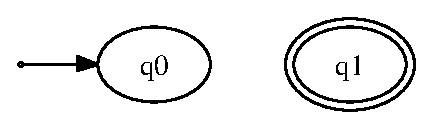
\epsfig{file=Abbildungen/aLeer.eps, scale=0.5}
      \caption{The \textsc{Fsm} $A(\emptyset)$.}
      \label{fig:aLeer.eps}
      \end{figure}
      Figure \ref{fig:aLeer.eps} shows the \textsc{Fsm} $A(\emptyset)$. It is obvious that we have
      $L\bigl(A(\emptyset)\bigr) = \{\}$. 
\item The \textsc{Fsm} $A(\varepsilon)$ is defined as
      \\[0.2cm]
      \hspace*{1.3cm}
      $A(\varepsilon) = \langle \{ q_0, q_1 \}, \Sigma, \{ \pair(q_0, \varepsilon) \mapsto q_1 \}, q_0, \{ q_1 \} \rangle$.


      \begin{figure}[!ht]
        \centering
      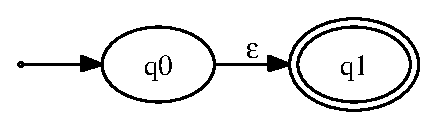
\epsfig{file=Abbildungen/aEpsilon.eps, scale=0.5}
      \caption{The \textsc{Fsm} $A(\varepsilon)$.}
      \label{fig:aEpsilon.eps}
      \end{figure}
      Figure \ref{fig:aEpsilon.eps} shows the \textsc{Fsm} $\varepsilon)$.
      We have that $L\bigl(A(\emptyset)\bigr) = \{\texttt{''}\}$, i.e. the automaton only accepts the empty string. 
\item For a letter $c \in \Sigma$ the \textsc{Fsm} $A(c)$ is defined as 
      \\[0.2cm]
      \hspace*{1.3cm}
      $A(c) = \langle \{ q_0, q_1 \}, \Sigma, 
                                \{ \langle q_0, c \rangle \mapsto q_1\}, q_0, \{ q_1 \} \rangle$.

      \begin{figure}[!ht]
        \centering
      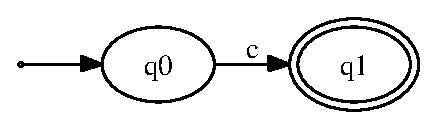
\epsfig{file=Abbildungen/aChar.eps, scale=0.5}
      \caption{The \textsc{Fsm} $A(c)$.}
      \label{fig:aChar.eps}
      \end{figure}
      Figure \ref{fig:aChar.eps} shows $A(c)$.
      We have that $L\bigl(A(c)\bigr) = \{c\}$, i.e. the automaton only accepts the character $c$. 
\item In order to define the \textsc{Fsm} $A(r_1 \cdot r_2)$ for the concatenation $r_1 \cdot r_2$ 
      we assume that the states in the \textsc{Fsm}s  $A(r_1)$ and $A(r_2)$ are different. 
      This can always be achieved by renaming the states of $A(r_2)$.
      Next, we assume that $A(r_1)$ and $A(r_2)$ have the following form:
      \begin{enumerate}
      \item $A(r_1) = \langle Q_1, \Sigma, \delta_1, q_1, \{ q_2 \}\rangle$,
      \item $A(r_2) = \langle Q_2, \Sigma, \delta_2, q_3, \{ q_4 \}\rangle$,
      \item $Q_1 \cap Q_2 = \{\}$.
      \end{enumerate}
      Then we can build the \textsc{Fsm} $A(r_1 \cdot r_2)$ from $A(r_1)$ and $A(r_2)$ as follows:
      \\[0.2cm]
      \hspace*{0.8cm}
       $A(r_1 \cdot r_2) := \langle Q_1 \cup Q_2, \Sigma, 
                \{ \pair(q_2,\varepsilon) \mapsto q_3 \} 
                   \cup \delta_1 \cup \delta_2, q_1, \{ q_4 \} \rangle$
      \\[0.2cm]
      Here, the notation $\{ \pair(q_2,\varepsilon) \mapsto q_3 \} \cup \delta_1 \cup \delta_2$ specifies that
      $A(r_1 \cdot r_2)$ contains all transitions from both $A(r_1)$ and $A(r_2)$ and, furthermore,
      contains an $\varepsilon$-transition from $q_2$ to $q_3$.     
      Formally, this transition function  $\delta$ can be specified as follows:
      \\[0.2cm]
      \hspace*{1.3cm}
      $\delta(q,c) := \left\{
      \begin{array}{ll}
        \{ q_3 \}       & \mbox{if $q = q_2$ and $c = \varepsilon$}, \\[0.2cm]
        \delta_1(q, c)  & \mbox{if $q \in Q_1$ and $\pair(q,c) \not= \pair(q_2,\varepsilon)$}, \\[0.2cm]
        \delta_2(q, c)  & \mbox{if $q \in Q_2$.} 
      \end{array}\right.
      $
      \\[0.2cm]


      \begin{figure}[!ht]
        \centering
      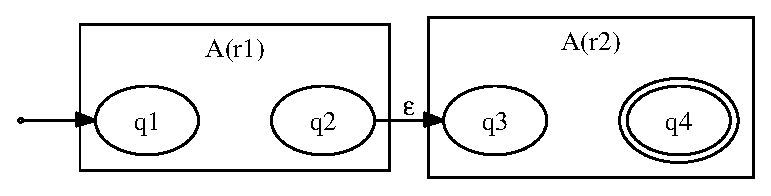
\epsfig{file=Abbildungen/aConcat.eps, scale=0.8}
      \caption{The \textsc{Fsm} $A(r_1 \cdot r_2)$.}
      \label{fig:aConcat.eps}
      \end{figure}
      Figure \ref{fig:aConcat.eps} shows the \textsc{Fsm} $A(r_1 \cdot r_2)$.

      Instead of having an $\varepsilon$-transition from $q_2$ to $q_3$ we can identify the states $q_2$ and
      $q_3$.  The advantage is that the resulting \textsc{Fsm} is smaller.
      We will do this when creating \textsc{Fsm}s by hand.

      I haven't done this identification in the definition above because both the graphical representation and 
      the implementation get more complicated when we identify these states.
\item In order to define the \textsc{Fsm} $A(r_1 + r_2)$ we assume again that the states of the \textsc{Fsm}s
      $A(r_1)$ and $A(r_2)$ are different and that $A(r_1)$ and $A(r_2)$ have the following form:
      \begin{enumerate}
      \item $A(r_1) = \langle Q_1, \Sigma, \delta_1, q_1, \{ q_3 \}\rangle$,
      \item $A(r_2) = \langle Q_2, \Sigma, \delta_2, q_2, \{ q_4 \}\rangle$,
      \item $Q_1 \cap Q_2 = \{\}$.
      \end{enumerate}
      Then the \textsc{Fsm} $A(r_1 + r_2)$ is defined as follows:
      \\[0.2cm]
      \hspace*{0.8cm}
       $\langle \{ q_0, q_5 \} \cup Q_1 \cup Q_2, \Sigma, 
                \{ \pair(q_0,\varepsilon) \mapsto q_1, \pair(q_0,\varepsilon) \mapsto q_2,
                   \pair(q_3,\varepsilon) \mapsto q_5, \pair(q_4,\varepsilon) \mapsto q_5 \} 
                   \cup \delta_1 \cup \delta_2, q_0, \{ q_5 \} \rangle$

      \begin{figure}[!ht]
        \centering
      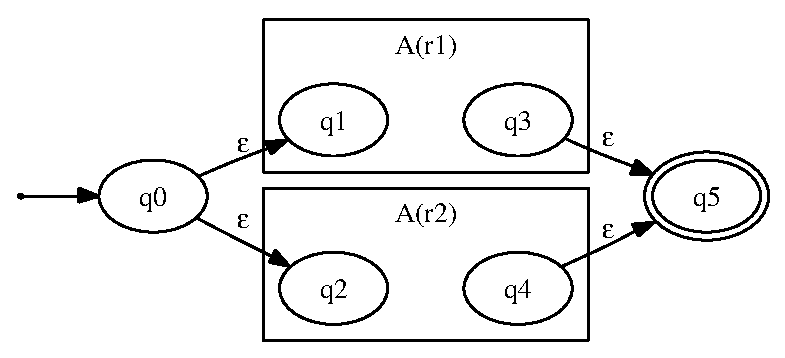
\epsfig{file=Abbildungen/aPlus.eps, scale=0.5}
      \caption{The \textsc{Fsm} $A(r_1 + r_2)$.}
      \label{fig:aPlus.eps}
      \end{figure}
      Figure \ref{fig:aPlus.eps} shows the \textsc{Fsm} $A(r_1 + r_2)$.
      In addition to the states of $A(r_1)$ and $A(r_2)$ there are two more states:
      \begin{enumerate}
      \item $q_0$ is the start state of the \textsc{Fsm} $A(r_1 + r_2)$,
      \item $q_5$ is the only accepting state of the \textsc{Fsm} $A(r_1 + r_2)$.
      \end{enumerate}
      In addition to the transitions of $A(r_1)$ and $A(r_2)$ the \textsc{Fsm} $A(r_1+r_2)$
      has four more $\varepsilon$-transitions.
      \begin{enumerate}
      \item The new start state $q_0$ has two
            $\varepsilon$-transitions leading to the start states $q_1$ and $q_2$ of the \textsc{Fsm}s
            $A(r_1)$ and $A(r_2)$.
      \item Each of the accepting states $q_3$ and $q_4$ of the \textsc{Fsm}s
             $A(r_1)$ and $A(r_2)$ has an $\varepsilon$-transition to the new accepting state $q_5$.
      \end{enumerate}
      In order to simplify this \textsc{Fsm} we could identify the three states
      $q_0$, $q_1$ and $q_2$ and the three states $q_3$, $q_4$ and $q_5$.  However, the resulting \textsc{Fsm}
      would be more difficult to understand and hence we are \underline{\red{not}} doing this when creating 
      \textsc{Fsm}s by hand.
\item In order to define the \textsc{Fsm} $A(r^*)$ we assume that
      \\[0.2cm]
      \hspace*{1.3cm}
      $A(r) = \langle Q, \Sigma, \delta, q_1, \{ q_2 \} \rangle$.
      \\[0.2cm]
      Then  $A(r^*)$ is defined as follows:
      \\[0.2cm]
      \hspace*{0.8cm}
       $\langle \{ q_0, q_3 \} \cup Q, \Sigma, 
                \{ \pair(q_0,\varepsilon) \mapsto q_1, \pair(q_2,\varepsilon) \mapsto q_1,
                   \pair(q_0,\varepsilon) \mapsto q_3, \pair(q_2,\varepsilon) \mapsto q_3 \} 
                   \cup \delta, q_0, \{ q_3 \} \rangle$.
      \\[0.2cm]


      \begin{figure}[!ht]
        \centering
      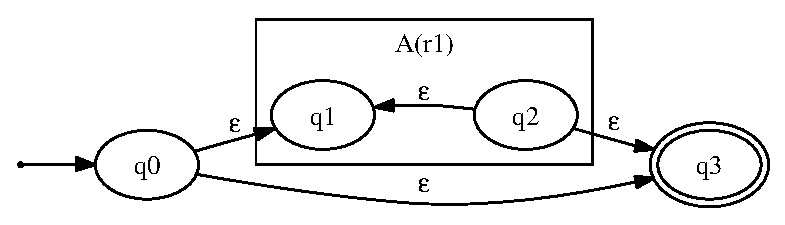
\epsfig{file=Abbildungen/aStar.eps, scale=0.5}
      \caption{The \textsc{Fsm} $A(r^*)$.}
      \label{fig:aStar.eps}
      \end{figure}
      Figure \ref{fig:aStar.eps} shows the \textsc{Fsm} $A(r^*)$.
      In comparison with $A(r)$ this \textsc{Fsm} has two additional states.
      \begin{enumerate}
      \item $q_0$ is the start state of $A(r^*)$,
      \item $q_3$ is the only accepting state of $A(r^*)$.
      \end{enumerate}
      The \textsc{Fsm} $A(r^*)$ has four more $\varepsilon$-transitions than $A(r)$: 
      \begin{enumerate}
      \item The new start state  $q_0$ has $\varepsilon$-transitions to the states
            $q_1$ and $q_3$.
      \item $q_2$ has an $\varepsilon$-transition back to the state $q_1$.
      \item $q_2$ also has an $\varepsilon$-transition to the state $q_3$.
      \end{enumerate}
      \textbf{\textcolor{red}{Attention}}:  If we would identify the two states 
      $q_0$ and $q_1$ and the two states $q_2$ and $q_3$, then the resulting \textsc{Fsm} would no longer be
      correct!
\end{enumerate}

The \textsl{Jupyter notebook}
\href{https://github.com/karlstroetmann/Formal-Languages/blob/master/Python/Regexp-2-NFA.ipynb}{regexp-2-NFA.ipynb} 
implements the theory discussed in this section.

\exerciseEng
Construct a non-deterministic \textsc{Fsm} that accepts the language specified by the regular expression
\\[0.2cm]
\hspace*{1.3cm}
$\texttt{a}^* \cdot \texttt{b}^*$.
\\[0.2cm]
Consider what would happen if you would identify the two states 
$q_0$ and $q_1$ and the two states $q_2$ and $q_3$ in step 6 of the construction given above. 
\eox

\exerciseEng
Construct a non-deterministic \textsc{Fsm} for the regular expression
\\[0.2cm]
\hspace*{1.3cm}
$(\texttt{a} + \texttt{b}) \cdot \texttt{a}^* \cdot \texttt{b}$.  
\eox



\section{\"Ubersetzung eines \textsc{EA} in einen regul\"aren Ausdruck}
Wir runden die Theorie ab, indem wir zeigen, dass sich zu jedem deterministischen endlichen
Automaten $A$ ein regul\"arer Ausdruck $r(A)$ angeben l\"asst, der dieselbe Sprache spezifiziert,
die von dem Automaten $A$ akzeptiert wird, f\"ur den also
\\[0.2cm]
\hspace*{1.3cm}
$L\bigl(r(A)\bigr) = L(A)$
\\[0.2cm]
gilt.  Der  Automat $A$ habe die Form
\\[0.2cm]
\hspace*{1.3cm}
$A = \langle \{ q_0, q_1, \cdots, q_n \}, \Sigma, \delta, q_0, F \rangle$.
\\[0.2cm]
F\"ur jedes Paar von Zust\"anden $\pair(p_1,p_2) \in Q \times Q$ definieren wir einen regul\"aren Ausdruck
$r(p_1, p_2)$.   Die Idee bei dieser Definition ist, dass der regul\"are Ausdruck
$r(p_1, p_2)$ alle die Strings $w$ spezifiziert, die den Automaten $A$ von dem Zustand
$p_1$ in den Zustand $p_2$ \"uberf\"uhren, formal gilt:
\\[0.2cm]
\hspace*{1.3cm}
$L\bigl(r(p_1, p_2)\bigr) = 
  \bigl\{ w \in \Sigma^* \mid \pair(p_1,w) \leadsto^* \pair(p_2, \varepsilon) \bigr\}$
\\[0.2cm]  
Die Definition der regul\"aren Ausdr\"ucke erfolgt \"uber einen Trick: Wir definieren f\"ur
$k=0,\cdots,n+1$ regul\"are Ausdr\"ucke $r^{(k)}(p_1, p_2)$.   Diese regul\"are Ausdr\"ucke
beschreiben gerade die Strings, die den Automaten $A$ von dem Zustand
$p_1$ in den Zustand $p_2$ \"uberf\"uhren, \underline{ohne} dass dabei zwischendurch ein
Zustand aus der Menge 
\\[0.2cm]
\hspace*{1.3cm}
$Q_k := \bigl\{ q_i \mid i \in \{k,\cdots,n \}  \bigl\} = \{ q_k, \cdots, q_n \}$ 
\\[0.2cm]
besucht wird.  Die Menge $Q_k$ enth\"alt also nur die Zust\"ande, deren Index gr\"o{\ss}er oder
gleich $k$ ist.  Formal definieren wir dazu die dreistellige Relation 
\\[0.2cm]
\hspace*{1.3cm}
$\mapsto_k \;\subseteq\; (Q \times \Sigma^* \times Q)$.
\\[0.2cm]
F\"ur zwei Zust\"ande $p, q \in Q$ und einen String $w$ soll 
\\[0.2cm]
\hspace*{1.3cm}
$p \stackrel{w}{\mapsto}_k q$
\\[0.2cm]
genau dann gelten, wenn der Automat $A$ von dem Zustand $p$ beim Lesen des Wortes $w$ in
den Zustand $q$ \"ubergeht, ohne dabei \underline{zwischendurch} in einen Zustand aus der
Menge $Q_k$ zu wechseln.  Mit ``zwischendurch'' ist hier gemeint, dass die Zust\"ande $p$
und $q$ sehr wohl in der Menge $Q_k$ liegen k\"onnen, nur die Zwischenzust\"ande d\"urfen nicht in $Q_k$
liegen.  Die formale Definition der Relation  
$p \stackrel{w}{\mapsto}_k q$ erfolgt durch Induktion nach der L\"ange des Wortes $w$:
\begin{enumerate}
\item[I.A.:] $|w| \leq 1$.  Im Induktions-Anfang haben wir zwei F\"alle:
  \begin{enumerate}
  \item $p \stackrel{\varepsilon}{\mapsto}_k p$,

        denn mit dem leeren Wort kann von $p$ aus nur der Zustand $p$ erreicht
        werden.
  \item $\delta(p, c) = q \;\Rightarrow\; p \stackrel{c}{\mapsto}_k q$,

        denn wenn der Automat beim Lesen des Buchstabens $c$ von dem Zustand $p$ direkt
        in den Zustand $q$ \"ubergeht, dann werden zwischendurch keine Zust\"ande aus $Q_k$
        besucht, denn es werden \"uberhaupt keine Zust\"ande zwischendurch besucht.
  \end{enumerate}
\item[I.S.:] $w = cv$ mit $|v| \geq 1$.

             \hspace*{1.3cm}
            $p \stackrel{c}{\mapsto} q \wedge q \not\in Q_k \wedge q \stackrel{v}{\mapsto}_k r
              \Rightarrow p \stackrel{cv}{\mapsto}_k r$.

             Wenn der Automat $A$ von dem Zustand $p$ durch Lesen des Buchstabens $c$
             in einen  Zustand $q \notin Q_k$ \"ubergeht und wenn der Automat dann von
             diesem Zustand $q$ beim Lesen von $v$ in den Zustand $r$ \"ubergehen kann, ohne
             dabei Zust\"ande aus $Q_k$ zu benutzen, dann geht der Automat beim Lesen von
             $cv$ aus dem Zustand $p$ in den Zustand $r$ \"uber,
             ohne zwischendurch in Zust\"ande aus $Q_k$ zu wechseln.
\end{enumerate}
Damit k\"onnen wir nun f\"ur alle $k=0,\cdots,n+1$ die regul\"aren Ausdr\"ucke
$r^{(k)}(p_1, p_2)$ definieren.  Wir werden diese regul\"aren Ausdr\"ucke so definieren, dass
hinterher
\\[0.2cm]
\hspace*{1.3cm}
$L\bigl(r^{(k)}(p_1, p_2)\bigr) = \bigl\{ w \in \Sigma^* \mid p_1 \stackrel{w}{\mapsto}_k p_2 \bigr\}$
\\[0.2cm]
gilt.
Die Definition der regul\"aren Ausdr\"ucke $r^{(k)}(p_1, p_2)$ erfolgt durch eine Induktion nach $k$.
\begin{enumerate}
\item[I.A.:] $k = 0$.  

  Dann gilt $Q_0 = Q$, die Menge $Q_0$ enth\"alt also alle Zust\"ande
  und damit d\"urfen wir, wenn wir vom Zustand $p_1$ in den Zustand $p_2$ \"ubergehen,
  zwischendurch \"uberhaupt keine Zust\"ande besuchen.

  Wir betrachten zun\"achst den Fall $p_1 \not= p_2$.  Dann kann $p_1 \stackrel{w}{\mapsto}_0 p_2$ nur dann gelten, wenn $w$ aus einem
  einzigen Buchstaben besteht.   Es sei
  \\[0.2cm]
  \hspace*{1.3cm}
  $\{ c_1, \cdots, c_l \} := \{ c \in \Sigma \mid \delta(p_1,c) = p_2 \}$
  \\[0.2cm]
  die Menge aller Buchstaben, die den Zustand $p_1$ in den Zustand $p_2$ \"uberf\"uhren.
  Falls diese Menge nicht leer ist, setzen wir 
  \\[0.2cm]
  \hspace*{1.3cm}
  $r^{(0)}(p_1, p_2) := c_1 + \cdots + c_l$. 
  \\[0.2cm]
  Ist die obige Menge leer, so gibt es keinen direkten \"Ubergang von
  $p_1$ nach $p_2$ und wir setzen 
  \\[0.2cm]
  \hspace*{1.3cm}
  $r^{(0)}(p_1, p_2) := \emptyset$.

  Wir betrachten jetzt den Fall $p_1 = p_2$.  Definieren wir wieder
  \\[0.2cm]
  \hspace*{1.3cm}
  $\{ c_1, \cdots, c_l \} := \{ c \in \Sigma \mid \delta(p_1,c) = p_1 \}$
  \\[0.2cm]
  als die Menge aller Buchstaben, die den Zustand $p_1$ in sich selbst \"uberf\"uhren,
  so k\"onnen wir in dem Fall, dass diese Menge nicht leer ist, 
  \\[0.2cm]
  \hspace*{1.3cm}
  $r^{(0)}(p_1, p_1) := c_1 + \cdots + c_l + \varepsilon$,
  \\[0.2cm]
  setzen.  Ist die obige Menge leer, so gibt es nur den \"Ubergang mit dem leeren Wort
  von $p_1$ nach $p_1$ und wir setzen 
  \\[0.2cm]
  \hspace*{1.3cm}
  $r^{(0)}(p_1, p_1) := \varepsilon$.
\item[I.S.:] $k \mapsto k+1$.  

  Bei dem \"Ubergang von $r^{(k)}(p_1, p_2)$ zu  $r^{(k+1)}(p_1, p_2)$ d\"urfen wir zus\"atzlich
  den Zustand $q_k$ benutzen, denn $q_k$ ist das einzige Element der Menge $Q_k$, das
  nicht in der Menge $Q_{k+1}$ enthalten ist.  Wird ein String $w$ gelesen, der
  den Zustand $p_1$ in den Zustand $p_2$ \"uberf\"uhrt, ohne dabei zwischendurch in einen
  Zustand aus der Menge $Q_{k+1}$ zu wechseln, so gibt es zwei M\"oglichkeiten:
  \begin{enumerate}
  \item Es gilt bereits $p_1 \stackrel{w}{\mapsto}_k p_2$.
  \item Der String $w$ kann so in mehrere Teile $w_1 s_1\cdots s_l w_2$ aufgeteilt werden,
        dass gilt
        \begin{itemize}
        \item $p_1 \stackrel{w_1}{\mapsto}_k q_k$,

               von dem Zustand $p_1$ gelangt der Automat also beim Lesen von $w_1$
               zun\"achst in den Zustand $q_k$, wobei zwischendurch der Zustand
               $q_k$ nicht benutzt wird.
        \item $q_k \stackrel{s_i}{\mapsto}_k q_k$ \quad f\"ur alle $i = \{ 1, \cdots, l\}$,

              von dem Zustand $q_k$ wechselt der Automat beim Lesen der Teilstrings
              $s_i$ wieder in den Zustand $q_k$.
        \item $q_k \stackrel{w_2}{\mapsto}_k p_2$,

              schlie{\ss}lich wechselt der Automat von dem Zustand $q_k$ in den Zustand
              $p_2$, wobei der Rest $w_2$ gelesen wird.
        \end{itemize}
        Daher definieren wir
        \\[0.2cm]
        \hspace*{1.3cm}
        $r^{(k+1)}(p_1,p_2) := 
         r^{(k)}(p_1,p_2) + 
         r^{(k)}(p_1,q_k) \cdot \bigl(r^{(k)}(q_k,q_k)\bigr)^* \cdot r^{(k)}(q_k,p_2)$.
        \\[0.2cm]
        Dieser Ausdruck kann wie folgt gelesen werden:  Um von $p_1$ nach $p_2$ zu kommen,
        ohne dabei zwischendurch Zust\"ande aus $Q_{k+1}$ zu benutzen, kann der Automat entweder direkt
        von $p_1$ nach $p_2$ gelangen, ohne zwischendurch Zust\"ande aus  $Q_k$ zu benutzen, was dem Ausdruck 
        $r^{(k)}(p_1,p_2)$ entspricht, oder aber der Automat wechselt von $p_1$ ein erstes Mal
        in den Zustand $q_k$, was den Ausdruck $r^{(k)}(p_1,q_k)$ erkl\"art, wechselt dann beliebig oft
        von $q_k$ nach $q_k$,  was den Ausdruck  $\bigl(r^{(k)}(q_k,q_k)\bigr)^*$ erkl\"art und wechselt
        schlie{\ss}lich von $q_k$ in den Zustand $p_2$, wof\"ur der Ausdruck $r^{(k)}(q_k,p_2)$ steht. 
  \end{enumerate}  
\end{enumerate}
Nun haben wir alles Material zusammen, um die Ausdr\"ucke $r(p_1,p_2)$ definieren zu k\"onnen.
Wir setzen 
\\[0.2cm]
\hspace*{1.3cm}
$r(p_1,p_2) := r^{(n+1)}(p_1,p_2)$. 
\\[0.2cm]
Dieser regul\"are Ausdruck beschreibt die W\"orter, die den Automaten von dem Zustand $p_1$ in
den Zustand $p_2$ \"uberf\"uhren, ohne dass der Automat dabei in einen Zustand der Menge
$Q_{n+1}$ wechselt.   Nun gilt aber
\\[0.2cm]
\hspace*{1.3cm}
$Q_{n+1} = \{ q_i | i \in \{0,\cdots,n \} \wedge i \geq n+1 \} = \{\}$,
\\[0.2cm]
die Menge ist also leer!  Folglich werden durch den regul\"aren Ausdruck $r^{(n+1)}(p_1,p_2)$
\"uberhaupt keine Zust\"ande ausgeschlossen:  Der Ausdruck beschreibt also genau die Strings,
die den Zustand $p_1$ in den Zustand $p_2$ \"uberf\"uhren, es gilt also
\\[0.2cm]
\hspace*{1.3cm}
$r^{(n+1)}(p_1,p_2) = r(p_1,p_2)$.
\\[0.2cm]
Um nun einen regul\"aren Ausdruck konstruieren zu k\"onnen, der die Sprache des Automaten $A$
beschreibt, schreiben wir die Menge $F$ der akzeptierenden Zust\"ande von $A$ als
\\[0.2cm]
\hspace*{1.3cm}
$F = \{ t_1, \cdots, t_m \}$
\\[0.2cm]
und definieren den regul\"aren Ausdruck $r(A)$ als
\\[0.2cm]
\hspace*{1.3cm}
$r(A) := r(q_0, t_1) + \cdots + r(q_0, t_m)$.
\\[0.2cm]
Dieser Ausdruck beschreibt genau die Strings, die den Automaten $A$ aus dem Start-Zustand
in einen der akzeptierenden Zust\"ande \"uberf\"uhren.
\qed
\vspace*{0.3cm}


\noindent
Damit sehen wir jetzt, dass die Konzepte ``\emph{deterministischer endlicher Automat}'' und
``\emph{regul\"arer Ausdruck}'' \"aquivalent sind.
\begin{enumerate}
\item Jeder deterministische endliche Automat kann in einen \"aquivalenten regul\"aren
      Ausdruck \"ubersetzt werden.
\item Jeder regul\"are Ausdruck kann in einen \"aquivalenten nicht-deterministischen endlichen Automaten
      transformiert werden.
\item Ein nicht-deterministischer endlicher Automat l\"asst sich durch die
      Teilmengen-Konstruktion in einen endlichen Automaten \"uberf\"uhren.
\end{enumerate}

\exercise
Konstruieren Sie f\"ur den in Abbildung \ref{fig:abstara.dot} gezeigten endlichen Automaten einen
\"aquivalenten regul\"aren Ausdruck.  


\solution
Der Automat hat die Zust\"ande $0$ und $1$.  Wir berechnen zun\"achst die regul\"aren Ausdr\"ucke
$r^{(k)}(i,j)$ f\"ur alle $i,j\in\{0,1\}$ der Reihe nach f\"ur die Werte $k =0$, $1$ und $2$:
\begin{enumerate}
\item F\"ur $k = 0$ finden wir:
      \begin{enumerate}
      \item $r^{(0)}(0, 0) = \texttt{a} + \varepsilon$,
      \item $r^{(0)}(0, 1) = \texttt{b}$,
      \item $r^{(0)}(1, 0) = \emptyset$,
      \item $r^{(0)}(1, 1) = \texttt{a} + \varepsilon$.
      \end{enumerate}
\item F\"ur $k=1$ haben wir:
      \begin{enumerate}
      \item F\"ur $r^{(1)}(0, 0)$ finden wir:
            \begin{eqnarray*}
                  r^{(1)}(0, 0) 
            & = & r^{(0)}(0, 0) + 
                  r^{(0)}(0, 0) \cdot \bigl(r^{(0)}(0, 0)\bigr)^* \cdot r^{(0)}(0, 0) \\
            & = & r^{(0)}(0, 0) \cdot \bigl(r^{(0)}(0, 0)\bigr)^*
            \end{eqnarray*}
             wobei wir im letzten Schritt die f\"ur regul\"are Ausdr\"ucke allgemeing\"ultige Umformung
             \\[0.2cm]
             \hspace*{1.3cm}
             $
             \begin{array}[t]{lcl}
               r + r \cdot r^* \cdot r & = & r \cdot (\varepsilon + r^* \cdot r) \\
                                       & = & r \cdot r^*
             \end{array}
             $
             \\[0.2cm]
             verwendet haben.
             Setzen wir f\"ur $r^{(0)}(0, 0)$ den oben gefundenen Ausdruck $\texttt{a} + \varepsilon$ ein, 
             so erhalten wir 
             \\[0.2cm]
             \hspace*{1.3cm}
             $r^{(1)}(0, 0) = (\texttt{a} + \varepsilon)\cdot (\texttt{a} + \varepsilon)^*$.
             \\[0.2cm]
             Wegen $(\texttt{a} + \varepsilon)\cdot (\texttt{a} + \varepsilon)^* = \texttt{a}^*$ haben
             wir insgesamt
             \\[0.2cm]
             \hspace*{1.3cm}
             $r^{(1)}(0, 0) = \texttt{a}^*$.
      \item F\"ur $r^{(1)}(0, 1)$ finden wir:
            \begin{eqnarray*}
                  r^{(1)}(0, 1) 
            & = & r^{(0)}(0, 1) + 
                  r^{(0)}(0, 0) \cdot \bigl(r^{(0)}(0, 0)\bigr)^* \cdot r^{(0)}(0, 1) \\
            & = & \texttt{b} + 
                  (\texttt{a} + \varepsilon) \cdot (\texttt{a} + \varepsilon)^* \cdot \texttt{b} \\
            & = & \texttt{b} + \texttt{a}^* \cdot \texttt{b} \\
            & = & (\varepsilon + \texttt{a}^*) \cdot \texttt{b} \\
            & = & \texttt{a}^* \cdot \texttt{b} 
        \end{eqnarray*}
      \item F\"ur $r^{(1)}(1, 0)$ finden wir:
            \begin{eqnarray*}
                  r^{(1)}(1, 0) 
            & = & r^{(0)}(1, 0) + 
                  r^{(0)}(1, 0) \cdot \bigl(r^{(0)}(0, 0)\bigr)^* \cdot r^{(0)}(0, 0) \\
            & = & \emptyset + \emptyset \cdot (\texttt{a} + \varepsilon)^* \cdot (\texttt{a} + \varepsilon) \\
            & = & \emptyset
            \end{eqnarray*}
      \item F\"ur $r^{(1)}(1, 1)$ finden wir
            \begin{eqnarray*}
                  r^{(1)}(1, 1)
            & = & r^{(0)}(1, 1) + 
                  r^{(0)}(1, 0) \cdot \bigl(r^{(0)}(0, 0)\bigr)^* \cdot r^{(0)}(0, 1) \\
            & = & (\texttt{a} + \varepsilon) + 
                  \emptyset \cdot (\texttt{a} + \varepsilon)^* \cdot \texttt{b} \\
            & = & (\texttt{a} + \varepsilon) + \emptyset  \\
            & = & \texttt{a} + \varepsilon  
            \end{eqnarray*}
      \end{enumerate}
\item F\"ur $k=2$ m\"ussen wir lediglich den regul\"aren Ausdruck $r^{(2)}(0, 1)$ berechnen.  Es gilt
            \begin{eqnarray*}
                  r^{(2)}(0, 1)
            & = & r^{(1)}(0, 1) + 
                  r^{(1)}(0, 1) \cdot \bigl(r^{(1)}(1, 1)\bigr)^* \cdot r^{(1)}(1, 1) \\
            & = & \texttt{a}^* \cdot \texttt{b} + 
                  \texttt{a}^* \cdot \texttt{b} \cdot (\texttt{a} + \varepsilon)^* \cdot (\texttt{a} + \varepsilon) \\
            & = & \texttt{a}^* \cdot \texttt{b} + \texttt{a}^* \cdot \texttt{b} \cdot \texttt{a}^* \\
            & = & \texttt{a}^* \cdot \texttt{b} \cdot (\varepsilon + \texttt{a}^*) \\
            & = & \texttt{a}^* \cdot \texttt{b} \cdot \texttt{a}^*.
        \end{eqnarray*}
\end{enumerate}
Da der Zustand 0 der Start-Zustand und der Zustand 1 der einzige akzeptierende Zustand
ist, k\"onnen wir nun den regul\"aren Ausdruck $r(A)$ angeben: 
\\[0.2cm]
\hspace*{1.3cm}
$r(A) = r^{(2)}(0, 1) = \texttt{a}^* \cdot \texttt{b} \cdot \texttt{a}^*$.
\\[0.2cm]
Dieses Ergebnis, das wir m\"uhevoll abgeleitet haben, h\"atten wir auch durch einen einfachen
Blick auf den Automaten erhalten k\"onnen, aber die oben gezeigte Rechnung formalisiert das,
was der ge\"ubte Betrachter unmittelbar erkennt und der beschriebene Algorithmus hat den
Vorteil, dass er sich implementieren l\"asst.
\qed

\exercise
Konstruieren Sie f\"ur den in Abbildung \ref{fig:exercise-13.eps} auf Seite
\pageref{fig:exercise-13.eps} gezeigten endlichen Automaten einen
regul\"aren Ausdruck, der dieselbe Sprache beschreibt, die von dem abgebildeten Automaten erkannt
wird.   

\begin{figure}[!ht]
  \centering
\epsfig{file=Abbildungen/exercise-13.eps, scale=0.5}
\caption{Ein deterministischer endlicher Automat.}
\label{fig:exercise-13.eps}
\end{figure}


\subsection{Implementing the Conversion of \textsc{FSM}s into Regular Expressions}
Figure \ref{fig:dfa-2-regexp.stlx} on page \pageref{fig:dfa-2-regexp.stlx} shows how to
implement the conversion of a finite state machine  into a regular expression.  We discuss
the details of this implementation next.

\begin{figure}[!ht]
\centering
\begin{Verbatim}[ frame         = lines, 
                  framesep      = 0.3cm, 
                  firstnumber   = 1,
                  labelposition = bottomline,
                  numbers       = left,
                  numbersep     = -0.2cm,
                  xleftmargin   = 0.8cm,
                  xrightmargin  = 0.8cm,
                ]
    dfa2RegExp := procedure(dfa) {
        [states, sigma, delta, q0, accepting] := dfa;
        return regexpSum({ rpq(q0, p, sigma, delta, states) : p in accepting });
    };
    regexpSum := procedure(s) {
        match (s) {
            case {}:
                 return 0;
            case { r }:
                 return r;
            case { r | rs }:
                 return Or(r, regexpSum(rs));
        }
    };
    rpq := procedure(p1, p2, sigma, delta, allowed) {
        match (allowed) {
            case {}: 
                 allChars := { c : c in sigma | delta(p1, c) == p2 };
                 sum := regexpSum(allChars);
                 if (p1 == p2) {
                     if (allChars == {}) {
                         return "";
                     } else {
                         return Or("", sum);
                     }
                 } else {
                     return sum;
                 }
            case { qk | restAllowed }:
                 rkp1p2 := rpq(p1, p2, sigma, delta, restAllowed);
                 rkp1qk := rpq(p1, qk, sigma, delta, restAllowed);
                 rkqkqk := rpq(qk, qk, sigma, delta, restAllowed);
                 rkqkp2 := rpq(qk, p2, sigma, delta, restAllowed);
                 return Or(rkp1p2, Cat(Cat(rkp1qk, Star(rkqkqk)), rkqkp2));
        }    
    };
\end{Verbatim}
\vspace*{-0.3cm}
\caption{Converting a \textsc{Dfa} into a regular expression.}
\label{fig:dfa-2-regexp.stlx}
\end{figure}

\begin{enumerate}
\item The function \texttt{dfa2RegExp} takes a deterministic finite state machine
      \texttt{dfa} as input.  For every accepting state $p$ of the given
      \texttt{dfa}, it calculates the regular expression $r(q_0,p)$, which describes those
      strings that transform the finite state machine from the start state $q_0$ into the
      state $p$.  If $\{p_1, \cdots, p_k\}$ is the set of all accepting states of
      \texttt{dfa}, then the regular expression
      \\[0.2cm]
      \hspace*{1.3cm}
      $r(q_0, p_1) + \cdots + r(q_0, p_k)$
      \\[0.2cm]
      describes the language accepted by \texttt{dfa}.  This regular expression is
      computed in line 3 via the two functions \texttt{regexpSum} and \texttt{rpq}.
\item The function \texttt{regexpSum} takes as input a set $s$ of regular expressions.
      If $s$ has the form
      \\[0.2cm]
      \hspace*{1.3cm}
      $\{ r_1, \cdots, r_k \}$,
      \\[0.2cm] 
      then the regular expression
      \\[0.2cm]
      \hspace*{1.3cm}
      $r_1 + \cdots + r_k$ 
      \\[0.2cm]
      is returned.  There are two special cases:
      \begin{enumerate}
      \item If $s$ is empty, then the regular expression $\emptyset$ is returned.
      \item If $s$ contains just one element, that is if $s$ has the form $s = \{r\}$, then $r$
            is returned.
      \end{enumerate}


\item The function \texttt{rpq} is called with 5 arguments:
      \begin{enumerate}
      \item The first two arguments $p_1$ and $p_2$ are states of a finite
            state machine.  The idea is that the call
            \\[0.2cm]
            \hspace*{1.3cm}
            \texttt{rpq(p1, p2, sigma, delta, allowed)}
            \\[0.2cm]
            computes the regular expression $r(\texttt{p1}, \texttt{p2})$, which is the
            expression that describes the set of those strings $s$ that take the
            finite state machine from the state \texttt{p1} to the state \texttt{p2}.
      \item \texttt{sigma} is the alphabet of the finite state machine.
      \item \texttt{delta} is the transition function of the finite state machine.
            In this program, we have chosen to represent \texttt{delta} as a \textsc{SetlX}
            \texttt{procedure} rather than as a binary relation.
      \item \texttt{allowed} is the set of all states that are allowed as intermediate states in the
             transition of the \textsc{Fsm} from the state $p_1$ into the state $p_2$.  This set
             corresponds to the set $\{q_0, q_1, \cdots, q_n\} - Q_{k}$ in the definition of the regular
             expression $r^{(k)}(p_1, p_2)$, i.e.~the set \texttt{allowed} is the complement of the
             set $Q_k$ with respect to the set of all states.
      \end{enumerate}
      The function \texttt{rpq} is defined by recursion on its last argument.  
      \begin{enumerate}
      \item The base case of the recursion is the case where the set \texttt{allowed} is
            empty.  Then the regular expression returned by the function \texttt{rpq} must
            only specify those strings that take the \textsc{Fsm} from the state $p_1$ to the state
            $p_2$ without visiting any other state in between.  
            In line 18, the function computes the set of all characters $c$ that take the \textsc{Fsm} from
            the state $p_1$ into the state $p_2$ directly, i.e.~that satisfy
            \\[0.2cm]
            \hspace*{1.3cm}
            $\delta(p_1, c) = p_2$.
            \\[0.2cm]
            If this set is given as $\{c_1, \cdots, c_k\}$, then the variable \texttt{sum}
            gets the value
            \\[0.2cm]
            \hspace*{1.3cm}
            $c_1 + \cdots + c_k$.
            \\[0.2cm]
            Of course, if the set $\{c_1, \cdots, c_k\}$ is empty, the sum 
            $c_1 + \cdots + c_k$ has to be interpreted as the regular expression
            $\emptyset$.
            Now there are two cases:
            \begin{enumerate}
            \item $p_1 = p_2$.  In this case, the empty string $\varepsilon$ transforms
                  the state $p_1$ into $p_2$ and therefore in this case the result returned  is
                  \\[0.2cm]
                  \hspace*{1.3cm}
                  $c_1 + \cdots + c_k + \varepsilon$.
            \item $p_1 \not= p_2$.  Then the result is given as
                  \\[0.2cm]
                  \hspace*{1.3cm}
                  $c_1 + \cdots + c_k$.
            \end{enumerate}
            The function \texttt{regexpSum} is used to compute the sum $c_1 + \cdots +c_k$.  It
            takes care to return $\emptyset$ if the set $\{c_1, \cdots, c_k\}$ is empty.
      \item In the recursive case, we arbitrarily pick a state $q_k$ from the set
            \texttt{allowed} of states that may be used to move from state $p_1$ to $p_2$.
            The state is removed from the set \texttt{allowed} to produce the set \texttt{restAllowed}.
            Then, the regular expression returned has the form
            \\[0.2cm]
            \hspace*{1.3cm}
            $r(p_1,p_2) + r(p_1,q_k) \cdot \bigl(r(q_k,q_k)\bigr)^* \cdot r(q_k,p_2)$.
            \\[0.2cm]
            Here, $r(p_1,p_2)$ is computed recursively as the regular expression that
            takes the \textsc{Fsm} from the state $p_1$ to the state $p_2$ using only the states
            from the set \texttt{restAllowed}.  The regular expressions 
            $r(p_1,q_k)$, $r(q_k,q_k)$, and $r(q_k,p_2)$ are defined in a similar way.
            The reasoning for returning this result is as follows:  In order to get from
            state $p_1$ to state $p_2$, there are two possibilities:
            \begin{itemize}
            \item If we do not need to visit the state $q_k$ when transforming  the \textsc{Fsm}
                  from state $p_1$ into state $p_2$, then the regular expression
                  \\[0.2cm]
                  \hspace*{1.3cm}
                  $r(p_1,p_2)$
                  \\[0.2cm]
                  already describes the transition.
            \item If we do need to visit the state $q_k$, then we move from $p_1$ to $p_2$
                  in three steps:
                  \begin{itemize}
                  \item We move from $p_1$ to $q_k$.
                  \item Next, we can move from $q_k$ to $q_k$ as many times as we wish.
                  \item Finally, we move from $q_k$ to $p_2$.
                  \end{itemize}
                  These three steps are summarized by the regular expression
                  \\[0.2cm]
                  \hspace*{1.3cm}
                  $r(p_1,q_k) \cdot \bigl(r(q_k,q_k)\bigr)^* \cdot r(q_k,p_2)$.
            \end{itemize}
      \end{enumerate}
\end{enumerate}


\paragraph{Historical Remark}
\href{http://en.wikipedia.org/wiki/Stephen_Cole_Kleene}{Stephen C.~Kleene} (1909 -- 1994) has shown in 1956 that the concepts of 
\emph{finite state  machines} and \emph{regular expression} have the same strength
\cite{kleene:1956}:  We have proven in this chapter that for every regular expression $r$ there is a
non-deterministic finite state machine $n$ such that $n$ recognizes the same set of strings that is
specified by $r$.  Next, we have seen that every non-deterministic finite state machine $n$ can be
transformed into a deterministic finite state machine $f$ which accepts the same language as $f$.
Finally, we have seen that given a finite state machine $f$ there is an algorithm to construct a
regular expression $r$ such that $r$ describes the language recognized by $f$.
Hence the notions of \emph{finite state machines} and \emph{regular expressions} are equivalent.

%%% Local Variables: 
%%% mode: latex
%%% TeX-master: "formal-languages.tex"
%%% End: 
